%% Adaptado a partir de :
%%    abtex2-modelo-trabalho-academico.tex, v-1.9.2 laurocesar
%% para ser um modelo para os trabalhos no IFSP-SPO

\documentclass[
    % -- opções da classe memoir --
    12pt,               % tamanho da fonte
    openright,          % capítulos começam em pág ímpar (insere página vazia caso preciso)
    %twoside,            % para impressão em verso e anverso. Oposto a oneside
    oneside,
    a4paper,            % tamanho do papel6. 
    % -- opções da classe abntex2 --schwinn
    % Opções que não devem ser utilizadas na versão final do documento
    %draft,              % para compilar mais rápido, remover na versão final
    paginasA4,  % indica que vai utilizar paginas em A4 
    %MODELO,             % indica que é um documento modelo então precisa dos geradores de texto
    %TODO,               % indica que deve apresentar lista de pendencias 
    % -- opções do pacote babel --
    english,            % idioma adicional para hifenização
    brazil              % o último idioma é o principal do documento
    ]{ifsp-spo-inf-cemi} % ajustar de acordo com o modelo desejado para o curso

% ---
% Pacotes básicos 
% ---
\usepackage[utf8]{inputenc}     % Codificacao do documento (conversão automática dos acentos)
% ---

%\usepackage{style}
        

% --- 
% CONFIGURAÇÕES DE PACOTES ADICIONAIS UTEIS
% --- 


% ---
% Informações de dados para CAPA e FOLHA DE ROSTO
% ---
\titulo{IFriends: uma comunidade virtual}

% Trabalho individual
%\autor{AUTOR DO TRABALHO}

% Trabalho em Equipe
% ver também https://github.com/abntex/abntex2/wiki/FAQ#como-adicionar-mais-de-um-autor-ao-meu-projeto
\renewcommand{\imprimirautor}{
\begin{tabular}{lr}
ANAÍ VILLCA ROJAS & SP3029085 \\
JAMILLI VITÓRIA GIOIELLI & SP3027473 \\
JOSÉ ROBERTO CLAUDINO FERREIRA & SP3024369 \\
JULIA ROMUALDO PEREIRA & SP3023061 \\
KAIKY MATSUMOTO SILVA & SP185075X \\
\end{tabular}
}


\disciplina{PDS - Prática para Desenvolvimento de Sistemas}

\preambulo{Projeto de sistema IFriends apresentado, conforme as normas ABNT, à disciplina de Prática para Desenvolvimento de Sistemas.}

\data{2022}

% Definir o que for necessário e comentar o que não for necessário
% Utilizar o Nome Completo, abntex tem orientador e coorientador
% então vão ser utilizados na definição de professor
\renewcommand{\orientadorname }{Professor:}
\coorientador{Carlos Henrique Verissimo Pereira}
\renewcommand{\coorientadorname}{Professor:}
\orientador{Johnata Souza Santicioli}


% ---


% informações do PDF
\makeatletter
\hypersetup{
        %pagebackref=true,
        pdftitle={\@title}, 
        pdfauthor={\@author},
        pdfsubject={\imprimirpreambulo},
        pdfcreator={LaTeX with abnTeX2 using IFSP model},
        pdfkeywords={abnt}{latex}{abntex}{abntex2}{IFSP}{\ifspprefixo}{trabalho acadêmico}, 
        colorlinks=true,            % false: boxed links; true: colored links
        linkcolor=blue,             % color of internal links
        citecolor=blue,             % color of links to bibliography
        filecolor=magenta,              % color of file links
        urlcolor=blue,
        bookmarksdepth=4
}
\makeatother
% --- 


% ----
% Início do documento
% ----
\begin{document}




% Retira espaço extra obsoleto entre as frases.
\frenchspacing 

%somente para o exemplo, fica primeiro
%\newcommand{\urlmodelosimples}{https://www.overleaf.com/project/58a3a66af9bb74023ba1bd56}

\newcommand{\urlmodelo}{\url{\urlmodelosimples}}

Esse documento foi feito a partir do modelo canônico do \abnTeX, o acesso ao PDF pode ser feito em 
\urlmodelo. A estrutura utilizada aqui foi um modelo utilizado no curso de Pós Graduação em Gestão de TI do \ac{ifsp}.
\todo[inline]{Remover texto informativo inicial}


Este documento não pode ser considerado como um padrão a ser seguido em sua totalidade, ele tem como maior objetivo demonstrar como utilizar o \LaTeX\ para obter um documento atendendo ao máximo o padrão do \ac{ifsp} e \ac{abnt}.

Faça leitura dos arquivos fonte \LaTeX\ e não somente do PDF gerado.

Esse documento é, em princípio, uma cópia do utilizado na disciplina de PDS e irá sofrer alterações durante o ano letivo. Essas alterações buscam induzir os alunos à prática com o \LaTeX\ . 

Algumas bibliotecas \LaTeX\ disponíveis no overleaf estão desatualizadas, para melhores resultados é recomendável a utilização de outro compilador utilizando as ultimas versões de todas bibliotecas.

Leia com cuidado :
\begin{itemize}
    \item \url{https://dicas.ivanfm.com/aulas/textos/};
    \item \url{https://dicas.ivanfm.com/aulas/textos/revisao-de-textos.html};
    \item exemplos no \autoref{cap-exemplos};
    \item \autoref{elementos-nao-textuais} sobre elementos não textuais que fala sobre o maior problema dos alunos que é de tentar posicionar as ilustrações.
\end{itemize}


\noindent\hrulefill


% -- lista de pendencias gerada pelo todonotes
% -- altere opções do usepackage para remover na versão final....
% \textit{\listoftodos
% \todo[inline]{remover lista de todo da versão final...}
% \newpage}

% ----------------------------------------------------------
% ELEMENTOS PRÉ-TEXTUAIS
% ----------------------------------------------------------
\pretextual

% ---
% Capa
% ---
\imprimircapa

\newcounter{todocounter}
\newcommand{\todonum}[2][]
{\stepcounter{todocounter}\todo[#1]{\thetodocounter: #2}}


% ---

% ---
% Folha de rosto
% (o * indica que haverá a ficha bibliográfica)
% ---
\imprimirfolhaderosto
%\imprimirfolhaderosto*
% ---

% -- resumo obrigatório
% ---
% RESUMOS
% ---

% resumo em português
\setlength{\absparsep}{18pt} % ajusta o espaçamento dos parágrafos do resumo
\begin{resumo}

O presente documento é o resultado obtido até a elaboração da \acs{POC} do projeto que visa a criação de uma comunidade virtual do \acs{ifsp} através do aprendizado adquirido na disciplina técnica de PDS no quarto ano do Curso Técnico de Informática, realizado no Instituto Federal de Educação, Ciência e Tecnologia de São Paulo, Campus de São Paulo. O objetivo central deste trabalho, desse modo, é apresentar a projeção e a implementação de uma prova de conceito de uma comunidade virtual qual visa a criação de um espaço de acolhimento de alunos para alunos. Propõe-se, assim, utilizar de um método ágil e de ferramentas de desenvolvimento para passar pelos processos de engenharia do sistema, além de estimular o trabalho em equipe. Sob essa perspectiva, o projeto pôde ser apresentado abordando seu tema principal e focando nas suas funcionalidades mais essenciais, como a gerenciamento das perguntas e a gerenciamento das respostas.


\textbf{Palavras-chaves}: Projeto. IFriends. Comunidade virtual.
\end{resumo}

% % resumo em inglês
% \begin{resumo}[Abstract]
% \begin{otherlanguage*}{english}
%   This is the english abstract.
% \todo[inline]{fazer tradução do resumo, não utilizar tradução automática}
%   \vspace{\onelineskip}

%   \noindent 
%   \textbf{Keywords}: Project. IFriends. Online Community.
%  \end{otherlanguage*}
% \end{resumo}


% ---
% inserir lista de ilustrações
% ---
\pdfbookmark[0]{\listfigurename}{lof}
\listoffigures*
\cleardoublepage
% ---

% ---
% inserir lista de quadros
% ---
\pdfbookmark[0]{\listofquadrosname}{loq}
\listofquadros*
\cleardoublepage
% ---

% ---
% inserir lista de abreviaturas e siglas
% ATENCAO o SHARELATEX/OVERLEAF GERA O GLOSSARIO SOMENTE UMA VEZ
% CASO SEJA FEITA ALGUMA ALTERAÇÃO NA LISTA DE SIGLAS É NECESSARIO UTILIZAR A OPÇÃO :
% "Clear Cached Files" DISPONIVEL NA VISUALIZAÇÃO DOS LOGS 
% ---
% https://www.sharelatex.com/learn/Glossaries


\ifdef{\printnoidxglossary}{
    \printnoidxglossary[type=\acronymtype,title=Lista de abreviaturas e siglas,style=siglas]
    \cleardoublepage
}{
}




% ---
% inserir o sumario
% ---
\pdfbookmark[0]{\contentsname}{toc}
\tableofcontents*
\cleardoublepage
% ---


% ----------------------------------------------------------
% ELEMENTOS TEXTUAIS
% ----------------------------------------------------------
\textual


% ----------------------------------------------------------
% Introdução (exemplo de capítulo sem numeração, mas presente no Sumário)
% ----------------------------------------------------------
\chapter{Introdução}
O presente documento é resultado da proposta de um projeto cujo objetivo é sustentado no planejamento e na execução de um sistema para a Web através do aprendizado obtido nas matérias técnicas do Curso Técnico de Informática, realizado no IFSP, e como forma de trabalho de conclusão de curso.

Tendo isto em vista e diante dos desafios presentes na lista de requisitos e orientações propostas para a iniciação deste projeto, os integrantes da equipe Bunka Bytes reuniram-se em busca de encontrar a solução que melhor se encaixasse em seus objetivos e nos da disciplina de \acs{pds}.

É pensando em soluções viáveis que a equipe voltou seu olhar para sistemas que contribuem para a criação de comunidades colaborativas na área de desenvolvimento de sistemas, que, segundo \citeonline{rosa2008identidade}, foi fortemente difundida pelas comunidades de Código Aberto (do inglês, \textsl{Open Source}), sendo primeiramente criada pela cultura \textsl{hacker}, na qual afirma que a paixão e o interesse dos \textsl{hackers} nas soluções foi uma das principais propulsoras do espírito colaborativo.

Além deles, foi trazido ao debate as possibilidades de aliar as principais dificuldades que os integrantes observaram durante sua vida acadêmica no \acs{ifsp}, a um sistema que pudesse suprir determinadas necessidades dos alunos, como os questionamentos que começam a surgir com mais frequência conforme o início dos estudos é dado, sendo eles em âmbitos diversos como: sobre a instituição de ensino, matérias e assuntos tratados no ensino médio, dúvidas sobre os conteúdos técnicos ou até mesmo a busca por um apoio educacional - como ocorrem nas monitoriais. 

O \gls{ifriends} surge nesse cenário, no qual a criação de uma comunidade de estudantes que colaborassem entre si, pudesse instigar o interesse dos alunos em ajudarem uns aos outros de maneira acessível e prática, onde uma dúvida estivesse a um palmo de distância.


\section{Objetivo}
%Nesta seção serão descritos os respectivos objetivos (principal e específico) pretendidos com a iniciação deste projeto. 
%\subsection{Objetivo Principal}

O objetivo deste projeto é tentar instigar o interesse dos estudantes que compreendem o \acs{ifsp} para poderem criar espaços colaborativos entre si, por um sistema onde os usuários interajam entre perguntas e respostas, fornecendo caminhos para o esclarecimento de suas dúvidas sobre a instituição de ensino, as áreas e disciplinas que a ela pertence.  

Dessa forma, o objetivo será aplicado através da construção de uma plataforma de perguntas, respostas e mentorias para a Web, em que qualquer usuário poderá submeter uma pergunta para ser respondida pelos outros membros da comunidade; além de possibilitar que estudantes possam escolher se tornar mentores sobre determinados assuntos, disponibilizando recursos para a criação de anúncios de eventos de monitorias (cuja localidade a eles deve competir) dentro de seus perfis de usuário. 

Tendo isso em vista e pensando numa melhor interatividade entre os usuários, o sistema deve passar por um processo de \gls{gamificação} em algumas de suas funcionalidades, como as votações para respostas e perguntas mais relevantes e os atributos dos usuários mais ativos  - assim como outros exemplos que devem ser adicionados durante o planejamento do projeto.


%\subsection{Objetivos Específicos}
%Dado o objetivo principal do projeto, o objetivo específico descrito nesta seção dá-se em forma de proposta de implementação do sistema citado anteriormente, na qual descrevemos um resumo da aplicação e seus propósitos, tendo em vista sua importância social e suas especificações técnicas. 


\section{Justificativa}
A reflexão com relação às formas complementares de aprendizagem é importante para a ampliação dos conteúdos interessados tanto aos alunos, quanto aos seus professores, pois permite que enxerguem, juntos, o ensino como um meio que evite a passagem de aprendizados de forma restrita e hierarquizada.

Por isso, \citeonline{fernandes2011redes} traz em sua pesquisa que o desafio da construção de sociedades de aprendizagem parte do pressuposto de que os recursos tecnológicos disponibilizados atualmente permitem aos estudantes aprenderem dentro e fora da escola e das mais variadas formas. Assim, para ele, a melhor forma se dá “construindo comunidades sustentadas pelo uso de tecnologias Web”.

O autor dá continuidade na exposição desse fenômeno ao atribuir o sucesso da potencialização da aprendizagem complementar e das relações sociais à ``Web 2.0''. Isto, pois, de acordo \citeonline{fernandes2011redes}, a mesma permitiu novas formas e possibilidades de criação de conteúdos e possibilitou o enfoque a uma aprendizagem motivada pelos interesses do aluno, em que ele deve assumir um papel exploratório nessa experiência, da qual poderá colher ensinamentos significativos, explica \citeonline{fernandes2011redes}.

Visando atrair atenção para o tema, o projeto tem como principal missão, permitir que os estudantes possam usufruir de uma ferramenta gratuita que proporcione a suavização do seu processo de aprendizagem, quando seus próprios colegas contribuirão com suas experiências passadas, além de deixarem um histórico para possibilitar um caminho menos árduo aos estudantes que virão. Por isso, espera-se que, com este projeto, a instituição de ensino também seja um agente na construção de uma comunidade propícia para estudantes, onde poderão unir-se em razão de dúvidas comuns, e assim incentivarem a disseminação de uma cultura colaborativa dentro de seus espaços.



\input{05-textos-proposta}
% Para facilitar a manutenção é sempre melhore criar um arquivo por capitulo, para exemplo isso não é necessário 

%---------------------------------------------------------------------------------------

%---------------------------------------------------------------------------------------


\chapter{Materiais e Métodos}
Segundo \citeonline{Junior:2010}, engenharia de \textsl{software} é ``um conjunto integrado de métodos e ferramentas utilizadas para especificar, projetar, implementar e manter um sistema'', e que, para tanto, reúne em si metodologias, métodos e ferramentas para que o projeto seja bem definido em todas as suas etapas, variando desde sua problemática inicial e indo até sua entrega enquanto um produto de \textsl{software}. É a partir disto, que \citeonline{Junior:2010} distingue um método de uma ferramenta:

\begin{citacao}

Um método é uma prescrição explícita de como chegar a uma atividade requerida por um modelo de ciclo de vida, visando otimizar a execução das atividades que foram especificadas. Já as ferramentas proporcionam apoio automatizado ou semi-automatizado aos métodos\cite{Junior:2010}.

\end{citacao}

Ademais, \citeonline{Junior:2010} ainda separa os métodos de desenvolvimento de sistema em três categoriais que permitem visualizar e solucionar o problema de diferentes maneiras para sua modelagem. Para a composição do presente projeto, no entanto, será utilizado como método principal a metodologia escolhida para a gestão do projeto e as ferramentas poderão ou não ser relacionadas a mesma, como há de ser especificado nas próximas seções.
%---------------------------------------------------------------
\section{Tecnologias e ferramentas de desenvolvimento}

Pensando no objetivo e alcance do projeto, decidimos por realizar uma aplicação Web inicialmente, a qual pode ser acessada de diferentes dispositivos de forma fácil, apenas sendo necessário o acesso à \textit{internet}. Outros fatores considerados são a experiência da equipe com o mesmo e a disponibilidade de conteúdo sobre desenvolvimento Web.

De modo a desenvolver essa aplicação, será usado \acs{html}, \acs{css} e JavaScript como base para o \textsl{\gls{front-end}}, já os \glspl{framework2} que servirão de auxílio serão o \gls{react-bootstrap} e o \gls{ant}. 

Para o \textsl{\gls{back-end}} foi considerada a linguagem Java, orientada a objetos; sua escolha foi feita pelo fato da equipe já possuir experiência com a linguagem, além de alguns já trabalharem com a mesma, ela também possui uma boa maturidade, contendo muitas informações disponíveis para ajudar no desenvolvimento. Em conjunto, será utilizado \textit{Spring Boot}: \gls{framework2} Java de código aberto, e será juntamente usado o \textit{Maven}: \gls{framework2} de automação e gerenciamento de dependências no projeto.  Já como padrão de desenvolvimento utilizado no  \textsl{\gls{back-end}}, será aplicado o padrão \acs{mvc}, que separa o projeto em três principais camadas, \textit{model}, \textit{view} e \textit{controller}.

No entanto, como arquitetura de sistema, foi escolhido utilizar a arquitetura \gls{REST API} na qual é possível separar o código \textsl{\gls{back-end}} do \textsl{\gls{front-end}} de maneira que as duas aplicações possam determinar a troca informações entre elas com requisições via protocolo \acs{http}. Está solução também é útil para escalonar a plataforma, já que a utilização de uma \acs{api} pode ser feita tanto por aplicações móveis, como para a Web.

\begin{figure}[htb]
\centering
\caption{Arquitetura Rest API}
\label{Arquitetura_Rest_API}
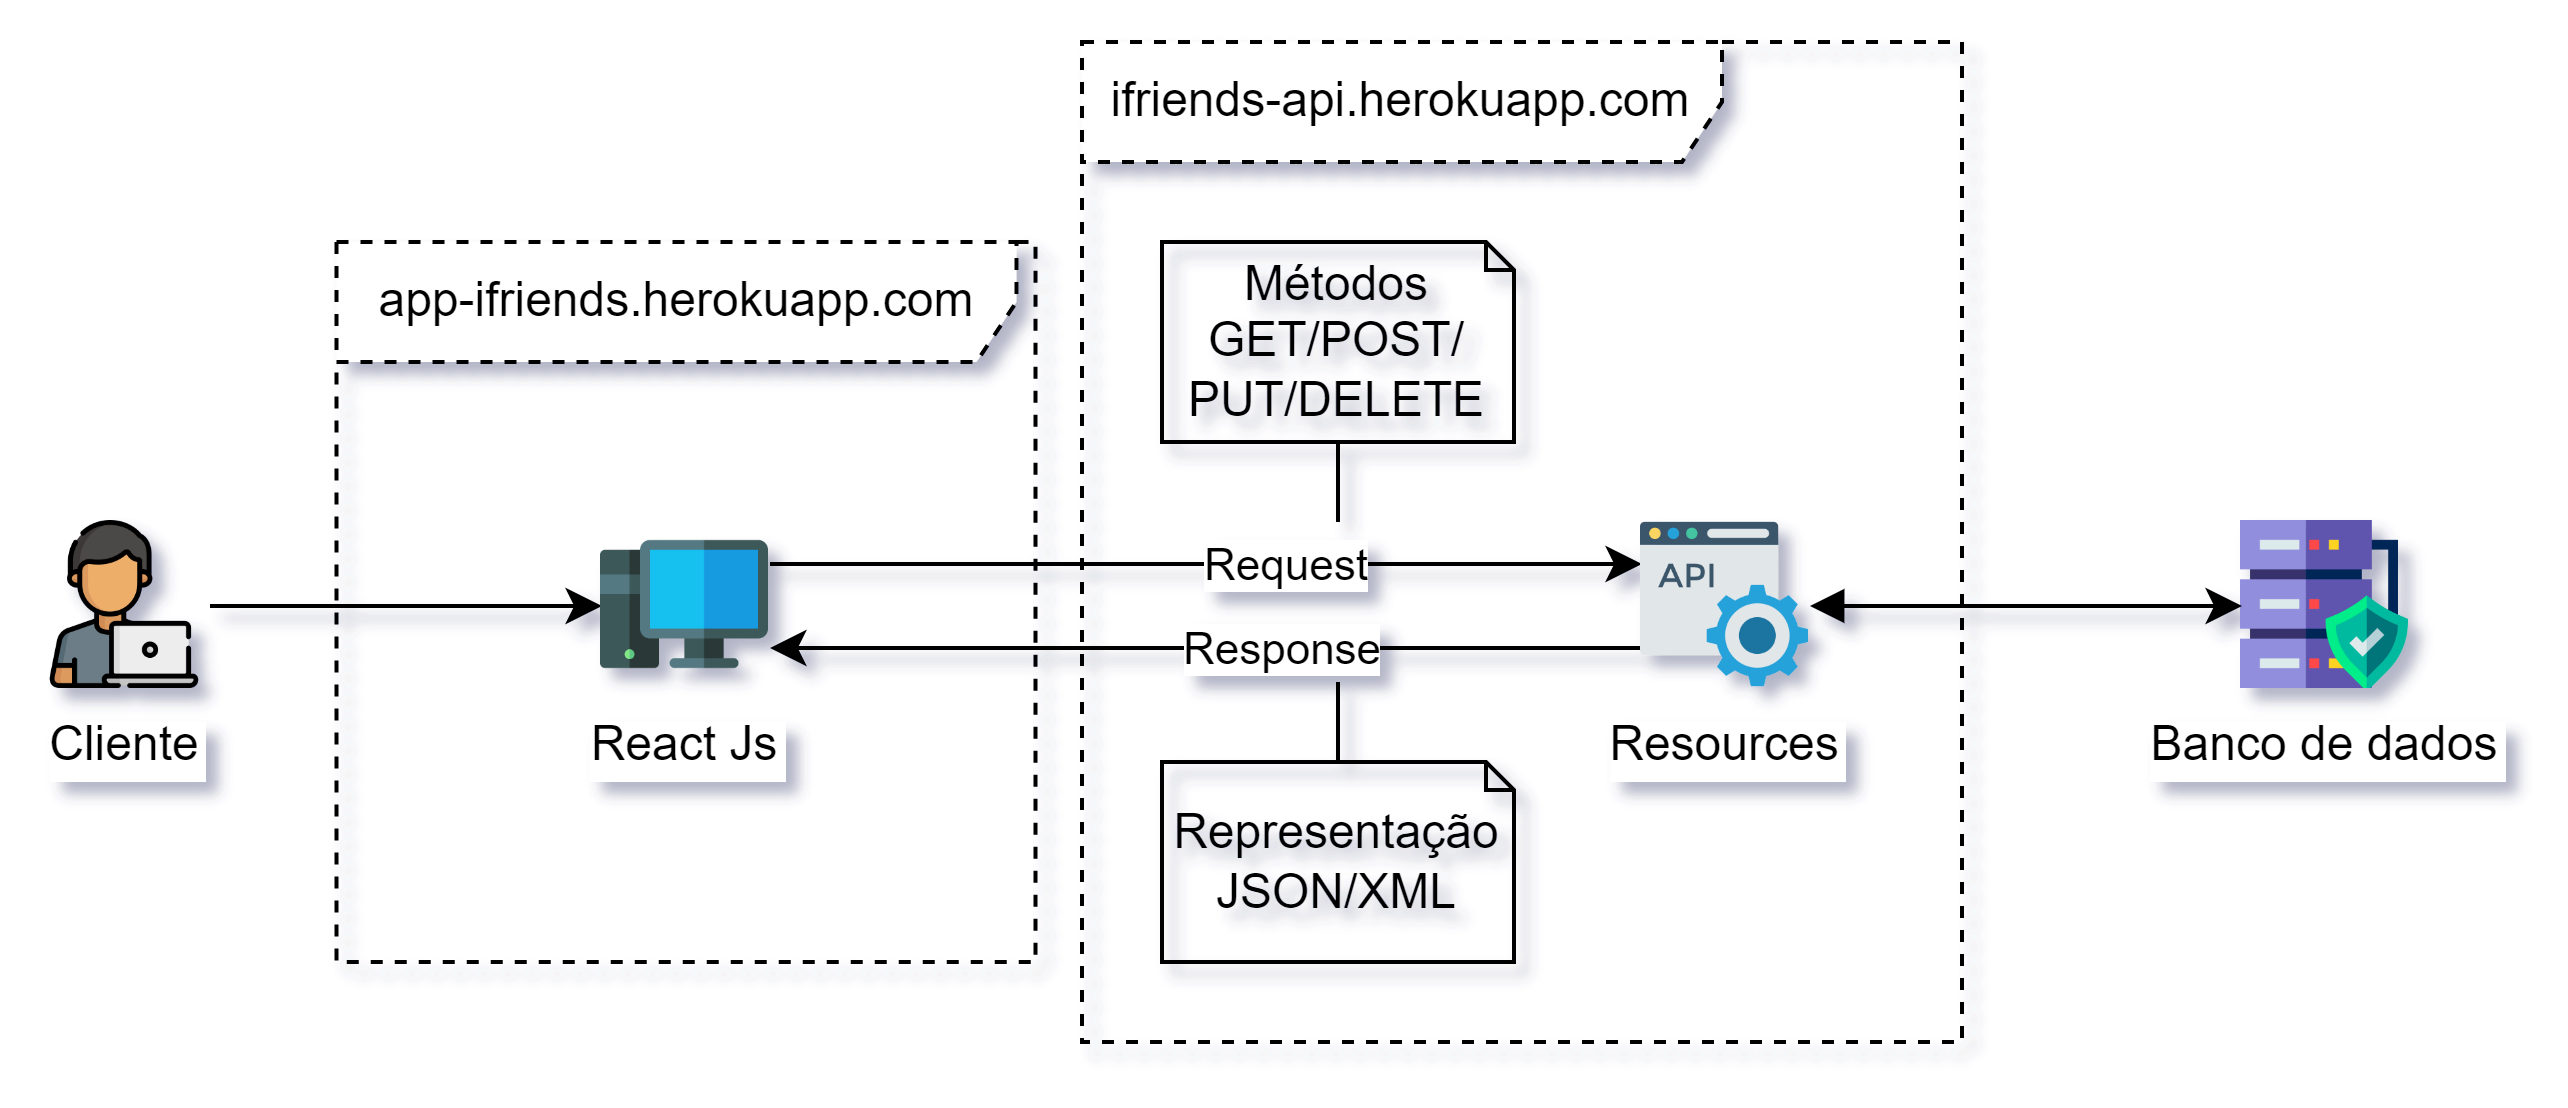
\includegraphics[width=1.0\textwidth]{anexos/Imagens_Diagramas/Arquitetura-Rest-API.png}
\fonte{Os autores.}
\end{figure}

Quanto ao banco de dados, será utilizado o \gls{postegreSQL}: um \acs{sgbd} popular de \acs{sql}, que serve para executar comandos no banco, como consultas, e alterações nos dados ou na estrutura.


Para hospedar a aplicação, será utilizado o \gls{heroku}, o qual é uma plataforma de nuvem que suporta diversas linguagens, que permite a implantação, escalonamento e gerenciamento do sistema.

Como inspiração para o sistema, será estudada sobre a plataforma \textit{Scoold}, a qual é uma aplicação  Web de código aberto de perguntas em respostas, inspirada no \textit{Stack Overflow}. Ela usa de base as mesmas tecnologias do projeto, tendo isso em vista, no caso da inviabilidade de seu uso, pode ser reaproveitado ideias implementadas nessa plataforma no seu código-fonte.

\subsection{Ferramentas de apoio}

Nesta seção serão especificados as ferramentas a serem utilizadas para a estruturação do sistema  Web.

\begin{itemize}
\item \textbf{Notion}: Foi escolhido como plataforma de organização de projetos, pois este possui métodos de gerenciamento de equipe, fornecendo uma interface para vários desenvolvedores trabalharem utilizando o quadro de kanban, assim como o compartilhamento de arquivos, vídeos e artigos; permitindo também notificações via e-mail sobre atualizações do projeto e de reuniões marcadas, por exemplo. 
    
\item \textbf{Discord}: Plataforma de comunicação online escolhida pela equipe, por ser a mais utilizada e conhecida entre os mesmos. Nela é possível criar servidores privados para compartilhar informações e realizar reuniões sobre o projeto.
    
\item \textbf{Overleaf}: Para a preparação do documento de visão, será usado o \LaTeX, visto que este possui comando de padronização para documentos acadêmicos, facilitando a sua construção, juntamente, com editor Overleaf que oferece um ambiente compartilhado entre os membros da equipe. 
    
\item \textbf{Figma}: Na parte de modelagem do sistema e elaboração ideias de soluções de problemas, escolheu-se o Figma, visto que é uma ferramenta gratuita que possui diversas opções de edição.
    
\item \textbf{Visual Studio Code}: A \acs{ide} escolhida para realizar a edição de código-fonte na parte \textsl{\gls{front-end}} do sistema, por razões de ser um recurso da atualidade com possibilidades de várias adaptações de ambiente, principalmente as nossas tecnologias escolhidas.

\item \textbf{Eclipse}: A \acs{ide} escolhida para realizar a edição de código-fonte na parte \textsl{\gls{back-end}}, por motivo de facilidade que o ambiente de desenvolvimento proporciona para rodar aplicações com Java e, também, seus recursos que fazem a integração com o banco de dados.
\end{itemize}



%---------------------------------------------------------------------------------------

%%%%%%%%%%%%%%%%%%%%%%%%%%%%%%%%%%%%%%%%
\section{Métodos de gestão e desenvolvimento}

Tendo em vista a organização do projeto \gls{ifriends}, a equipe escolheu utilizar os princípios e valores do Manifesto Ágil como norteadores nos seus processos de planejamento, modelagem e desenvolvimento do projeto. Deste modo, elencou-se  o \gls{framework} Scrum como metodologia ágil que irá servir como referência para o trabalho da Bunka Bytes.

\subsection{Metodologia ágil: Scrum} 
Segundo \citeonline{ambler2004modelagem}, o termo “metodologias ágeis” surgiu em fevereiro de 2001, quando  especialistas em processos de engenharia de \textsl{software} se reuniram e estabeleceram princípios comuns entre todas as metodologias, criando a Aliança Ágil e o estabelecimento do ``Manifesto Ágil'' \textsl{(Agile Manifesto)}.

O termo metodologia ágil consiste na otimização do tempo para a realização de determinado projeto, visando a rapidez na entrega e na qualidade do mesmo, surgindo assim, como uma resposta mais leve, mais assertiva e menos custosa em relação aos métodos pesados que eram utilizados para a construção de sistemas. Nas metodologias ágeis, os processos, as ferramentas, as documentações, as negociações e os planejamentos, possuem prioridade secundária, pois os indivíduos e suas interações são considerados essências e indispensáveis \cite{sganderla2016aprimorando}.

Para isso, o manifesto determina quatro valores principais, sendo eles: o enfoque nos indivíduos e nas interações, e não nos processos ou algoritmos; a adaptação e maior flexibilidade a novos fatores decorrentes do desenvolvimento do projeto; o foco na funcionalidade do sistema e na documentação mais simples e objetiva, e por último, a preferência por um ambiente de trabalho mais colaborativo e menos burocrático  \cite{sganderla2016aprimorando}. 

Segundo \citeonline{cruz:2018}, o Scrum pode ser definido como ``um \textsl{\gls{framework}} para desenvolver e manter produtos complexos que também pode ser utilizado no gerenciamento ágil de projetos que se destinam também à criação de produtos''. Neste caso, sabida a escolha da utilização de uma metodologia ágil para o gerenciamento do presente projeto, foi decidido aplicá-la com base no Scrum e suas especificações, porém, como a finalidade do trabalho é acadêmica, resolveu-se adaptar algumas de suas características para que a metodologia pudesse ser implementada como uma referência na organização e gestão do projeto. Estas, por conseguinte, serão explicitadas mais a frente, conforme apresentadas as particularidades do \textsl{\gls{framework}}.

Dentre as principais características do Scrum, está a divisão do desenvolvimento em ciclos repetitivos e curtos, permitindo modificações, adaptações e correções no produto de forma iterativa e incremental, o que, segundo \citeonline{cruz:2018} permite encontrar desvios mais rápido e com menos impacto. \citeonline{cruz:2018} explica que para que os processos sejam otimizados de tal forma, o Scrum possui ainda três pilares de sustentação: transparência, a inspeção e a adaptação.


Além dos pilares da metodologia, há cinco valores importantes para sua construção e prática durante um projeto: coragem, foco, comprometimento, respeito e abertura.  De acordo com \citeonline{cruz:2018} os valores do Scrum são responsáveis por reforçar os princípios do manifesto ágil, principalmente considerando o comportamento e as pessoas maiores do que os processos e ferramentas. 

%--------------------------------------------------------
\subsubsection{O quadro de kanban}

Segundo \citeonline{peinado2007compreendendo}, o nome Kanban vem do japonês ``cartão'' e a sua origem deu-se pela seguinte razão:

\begin{citacao}
Este nome surgiu em razão do sistema de controle visual dos estoques de materiais, pois são frequentemente utilizados cartões para representar os contentores cheios ou vazios, estes cartões são retirados ou colocados em um quadro à medida que o material é utilizado, ou reposto
\cite{peinado2007compreendendo}.
\end{citacao}
%%%%%%%%%%%%%%%%%%%%%%%%%%%
E através da implantação realizada por \citeonline{silva2012beneficios}, devido aos problemas e necessidades encontrados ao longo dos \textsl{sprints}, houve a criação de um processo ágil, baseado nas práticas do Scrum com características do Kanban:

\begin{citacao}
As tarefas ou itens de trabalho foram representadas através de cartões (do inglês \textsl{post-its}) fixados em um quadro (do inglês \textsl{cardwall}). 
Esse quadro, por sua vez, era dividido em colunas que representavam as fases do fluxo de trabalho (do inglês \textsl{workflow}) da equipe. 
As tarefas eram distribuídas sequencialmente nas colunas à medida que avançavam no fluxo de trabalho \cite{silva2012beneficios}.
\end{citacao}

No projeto  a implementação do kanban foi similar, porém todo o esquema presencial foi adaptado ao quadro remoto. Para conciliar a participação continua da equipe, a ferramenta \textsl{Notion} é utilizada como auxiliar aos processos de organização, onde também foi possível criar o quadro de kanban do projeto. 

O quadro de kanban usado pela equipe Bunka Bytes, responsável pelo projeto apresenta 5 colunas, nas quais são representadas visualmente em qual estagio a tarefa se encontra, as colunas se classificam como ``para fazer'', ``planejamento'', ``em andamento'', ``para revisar'' e ``feito''. E por ``cartões virtuais'' são colocadas as tarefas no quadro.

Foi decidido utilizar uma classificação em ordem de prioridade para cada tarefa, podendo ser "alta", representada pela cor vermelha, ``média'', representada pela cor laranja, e ``baixa'' representada pela cor verde, tais prioridades são atribuídas às tarefas assim que a \textsl{sprint} é definida.


De maneira geral, o uso do quadro de kanban é beneficial ao projeto, já que através de sua aplicação a equipe consegue conciliar de maneira clara e precisa as tarefas compartilhadas. A utilização do quadro remotamente, faz com que a equipe possa ainda acessá-lo de qualquer lugar, facilitando o processo de transparência dos itens e faz com que todos tenham em usas mão as atividades a serem feitas, podendo ajustá-las no momento em que preferirem. 

%------------------------------------------------



\subsection{Gestão da equipe}
A equipe Scrum é composta por três papéis: o \textsl{Scrum Master}, o \textsl{Product Owner} e o Time de Desenvolvimento:

\begin{citacao}

O primeiro, chamado \textsl{Scrum Master}, é considerado o responsável por garantir que o Scrum seja entendido e aplicado, para que o Time Scrum esteja aderindo os valores, as práticas e as regras do Scrum, e, portanto, trabalha como um líder ou técnico da equipe. Já o \textsl{Product Owner}, é o principal responsável pelo gerenciamento do \textsl{backlog} do produto, por garantir o valor do trabalho realizado pelo Time, e pela satisfação e atendimento das necessidades do cliente. O Time de Desenvolvimento, por outro lado, é responsável por executar o desenvolvimento e transformar o \textsl{backlog} do produto em incrementos de funcionalidades, criando um sistema pronto que possa ser entregue ao cliente \cite{cruz:2018}.

\end{citacao}

Portanto, para fins de organização, o Time de Desenvolvimento poderá ser dividido em subequipes, sendo elas: desenvolvimento ( \textsl{\gls{front-end}} e \textsl{\gls{back-end}}), design e documentação, e mídias. Nelas, estão inclusas as funções de programadores \textsl{\gls{front-end}} e \textsl{\gls{back-end}}, divididas entre os integrantes Jamilli Vitória Gioielli, José Roberto Claudinho Ferreira e Kaiky Matsumoto Silva; sendo a Jamilli responsável por supervisionar o \textsl{\gls{front-end}} da aplicação, e o José (que também auxiliará no \textsl{\gls{front-end}}) juntamente com o Kaiky pelo \textsl{\gls{back-end}} - que também inclui a administração do banco de dados. 

Além dessas, as outras duas subequipes foram dividias entre as integrantes Anaí Villca Rojas, responsável  por supervisionar o design de experiência/interface de usuário; e Julia Romualdo Pereira, responsável pelo gerenciamento da documentação e das mídias do projeto (como o canal no \gls{youtube} e as postagens no Blog). 

 De todo modo, a documentação e as mídias do projeto deverão ser revisadas, obrigatoriamente, por todo o time, de modo a manter um conhecimento sobre a aplicação melhormente distribuída. Entretanto, precisa-se compreender que a modelagem de dados e a elicitação de requisitos da aplicação serão feitas com o auxílio de todos os integrantes, visto que são partes de extrema importância para que a compreensão de todos sobre o cenário corresponda com o objetivo principal pretendido. No \autoref{distribuicao_tarefas}, é possível observar uma relação das supervisões dos integrantes em cada área do projeto. 

%%%%inserir tabela de relação das tarefas dos integrantes
\begin{quadro}[htb]
\centering
\ABNTEXfontereduzida
\caption{Distribuição de tarefas}
\label{distribuicao_tarefas}
\resizebox{\linewidth}{!}{

\begin{tabular}{|l|c|c|c|c|}
\hline

\thead{Responsável} & \thead{Front-end} & 
\thead{Back-end}  & \thead{Documentação e Mídias} & \thead{Design}\\
\hline
Anaí &    &    & \circlemark & \circlemark \\
\hline
Jamilli & \circlemark &  &  & \circlemark \\
\hline
José & \circlemark & \circlemark &  &   \\
\hline
Julia &  &  &  \circlemark &  \\
\hline
Kaiky & & \circlemark &  &  \\
\hline


\end{tabular}}\legend {Fonte: Os autores.}
\end{quadro}
\FloatBarrier 

Entretanto, é importante salientar que as funções atribuídas a cada um não são exclusivas e podem variar conforme a necessidade de entrega do projeto. As subequipes são de responsabilidade de todos os integrantes e apenas foram divididas assim para fins de organização das tarefas do projeto. Levando isso em consideração, as funções de \textsl{Scrum Master ou Iteration Manager} e \textsl{Product Owner} foram adaptadas, ainda que não seja o ideal na metodologia ágil, para um único papel, representado pela integrante Jamilli Vitória Gioielli. Porém, vale ressaltar ainda que, nesse modelo escolhido, toda a equipe é responsável pela inspeção dos processos do projeto, e não somente o \textsl{Scrum Master ou Iteration Manager}:

\begin{citacao}

O Time deve ser multidisciplinar e multifuncional, possuindo todo o conhecimento necessário para criar um incremento no trabalho. [...] Não há títulos no Time, e não há exceção a esta regra. Não deve existir distinção de cargos ou funções, títulos ou senioridades, e muito menos áreas determinadas ou específicas de atuação. No Scrum todos os integrantes do Time são conhecidos como “desenvolvedores”.

Individualmente os integrantes do Time de Desenvolvimento podem ter habilidades específicas, mas, independentemente disso, a responsabilidade a respeito de uma entrega continua sendo do Time de Desenvolvimento como um todo \cite{cruz:2018}.

\end{citacao}

Para organizar a produtividade continua de desenvolvimento do projeto, buscando seguir uma das vertentes propostas na metodologia ágil de entregas semanais, a equipe criou um cronograma de entregas por aula baseado a partir do plano de ensino da disciplina disponibilizado pelos orientadores, ou seja, a equipe busca realizar durante a semana a atividade proposta para a aula seguinte para aproveitar o tempo em sala de aula validando o que foi realizado com os orientadores. 

O cronograma de entrega semanal utilizado para o desenvolvimento do projeto \gls{ifriends} pode ser observado na \autoref{cronograma_desenvolvimento}.

\begin{figure}[htb]
\centering
\caption{Cronograma de Desenvolvimento Semanal}
\label{cronograma_desenvolvimento}
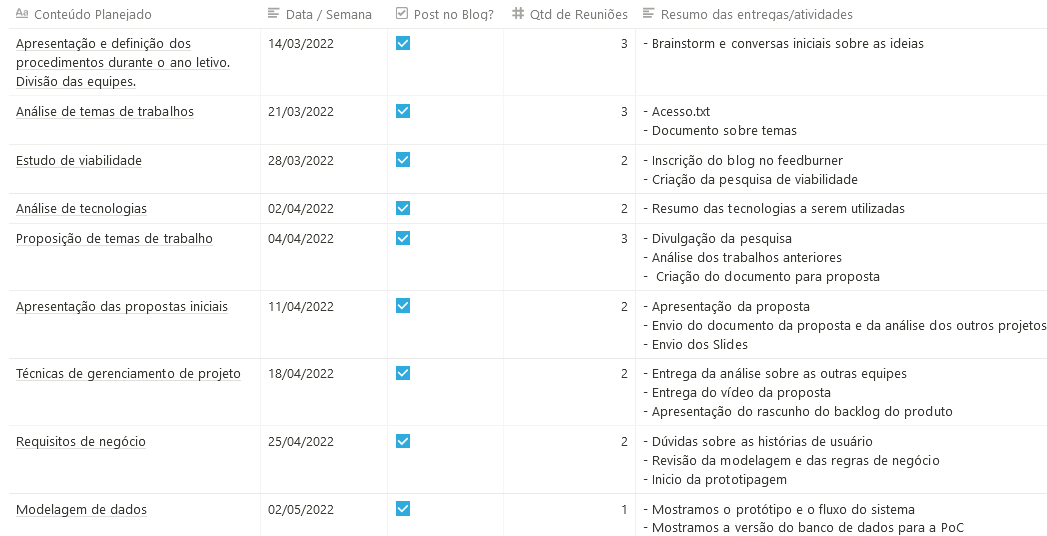
\includegraphics[width=1.0\textwidth]{anexos/Imagens_proposta/cronograma_desenvolvimento.png}
\fonte{Os autores.}
\end{figure}
\FloatBarrier

\subsection{Desenvolvimento: artefatos e eventos}

Tendo em vista a finalidade acadêmica do projeto, foi estipulado um valor mínimo de duas reuniões semanais dedicadas na construção do mesmo, levando em conta a organização individual de cada membro da equipe, além da priorização para que a tomada de decisões e planejamentos sejam feitas no dia das aulas da disciplina de \acs{pds}. Sobre os artefatos e eventos do Scrum, lista-se a seguir suas funcionalidades originais, descritos por \citeonline{cruz:2018}, e como serão adaptados:

\begin{itemize}
\item \textsl{Backlog}: é descrito como uma lista de todas as características, funções, tecnologias, melhorias e correções que constituem o produto a ser entregue. É também subdividido em ``do produto'', ``da versão de entrega'' e ``da \textsl{Sprint}'';

\item \textsl{Sprint}: originalmente pensada para durar um mês ou menos e possuir uma meta estabelecida com um objetivo claro, foi pensada 
para durar até duas semanas, já que as orientações da disciplina exigem que existam entregas frequentes, isto é, todas as semanas. Portanto, o ideal é que se dê início ao trabalho a ser entregue pelo menos uma semana antes de sua entrega;

\item \textsl{Time-boxed}: é esperado que o tempo estipulado para executar uma tarefa seja cumprido e que o trabalho proposto, seja realizado. Tendo em vista os curtos prazos,
também poderá ser adaptado conforme a entrega;

\item Planejamento da \textsl{Sprint}: ainda será utilizado para definir ``o que será feito'' e ``como'', porém, ao contrário das oito horas mínimas 
estipuladas, a equipe definiu um mínimo de duas horas para tal reunião, que poderá acontecer nas segundas-feiras, durante a aula de \acs{pds} ou aos finais de semana, logo após a finalização dos entregáveis;

\item Reuniões Diárias: não serão mantidas de maneira síncrona, visto que cada membro da equipe possui horários de disponibilidade diferentes. Porém, poderão ocorrer de forma assíncrona, de modo a compreender se existem impedimentos durante a execução das tarefas planejadas para a semana;

\item Revisão da \textsl{Sprint}: seu maior objetivo é a revisão do \textsl{Product Owner}, ou do cliente, em todos os itens concluídos pelo Time. Porém, 
não terá \textsl{Time-boxed} de quatro horas, visto que a aprovação dos professores orientadores (o cliente) pode ser mais rápida e acontecer durante a execução das tarefas. No entanto, o Time a realizará em todo final de entrega, para que os retornos dos professores levem em consideração o trabalho final;

\item Retrospectiva da \textsl{Sprint}: possui originalmente \textsl{Time-boxed} de até três horas e é feita para identificação 
de medidas de melhoria no processo do time que serão aplicadas na próxima \textsl{Sprint}. Foi escolhido adaptá-la para acontecer às terças-feiras, antes do início das aulas, para que as entregas feitas às segundas-feiras estejam frescas e o processo realizado pelo time possa ser melhor avaliado para a melhoria contínua.
\end{itemize}


Para a definição do \textsl{backlog} do produto, o Scrum conta com um recurso chamado histórias de usuário, que pode ser definido como: 

\begin{citacao}

História é uma descrição resumida, porém clara e objetiva, de alguma funcionalidade que deverá ser fornecida pelo produto a ser entregue, sempre do ponto de vista do usuário final. Uma história não é uma especificação completa da funcionalidade, mas uma promessa de discutir uma funcionalidade, ou, simplesmente, um lembrete de que a discussão já aconteceu. Um modelo simples de como escrever uma história seria: “Como um <tipo de usuário>, eu quero <um objetivo> para que <atenda a uma necessidade>.” \cite{cruz:2018}

\end{citacao}

Entretanto, vale ressaltar que as histórias de usuário do presente projeto serão montadas somente na parte de desenvolvimento, isto é, quando o produto começar a ser construído pelo Time Scrum e após os principais itens de \textsl{backlog} estarem descritos. Como ainda se encontra na fase de planejamento e modelagem, tal recurso ainda não foi acionado no projeto.

Outra ressalva diz respeito a utilização do \textsl{Scrum Poker} ou \textsl{Planning Poker Card}, que, segundo \citeonline{cruz:2018}, é definido como ``uma técnica que auxilia na estimativa de histórias e tarefas com base no consenso de todo o Time''. Para tanto, o Time utiliza um conjunto de cartas com valores representando os pontos ou horas por história. Sobre o funcionamento do \textsl{Planning Poker Card}:

\begin{citacao}

O seu uso é simples: o \textsl{Product Owner} ou um membro do Time apresenta a história, ou tarefa. Após uma breve discussão, cada um escolhe uma carta e a coloca virada sobre uma mesa, de forma que um não constate o valor da carta que o outro escolheu. Quando todos colocarem suas cartas, elas são desviradas para que todos vejam os valores.

Caso não haja consenso entre as cartas escolhidas, as diferenças são discutidas brevemente e uma nova rodada acontece, até que haja convergência e consenso.\cite{cruz:2018}

\end{citacao}

Para o presente projeto, no entanto, o \textsl{Planning Poker Card} será utilizado durante o processo de desenvolvimento do produto e após as histórias de usuário da \textsl{sprint} estarem bem descritas. Vale ressaltar que este processo é apenas para estimar o trabalho da equipe e pode variar conforme o andamento do projeto.
%%%%%%%%%%%%%%%%%%%%%%%%%%%%%%%%%%



%---------------------------------------------------------------------------------------



%--------------------------------------------------------------------------------
\chapter{Desenvolvimento}
  Baseando-se na conceituação de engenharia de \textsl{software} dada por \citeonline{SOMMERVILLE:2019}, neste capítulo é descrito o desenvolvimento do sistema, cujas etapas estão apoiadas em técnicas que vão desde sua especificação até sua evolução. Neste sentido, \citeonline{SOMMERVILLE:2019} destaca quatro etapas como fundamentais para os processos de \textsl{software}, sendo elas sequenciadas em: especificação, desenvolvimento, validação e evolução. As etapas correspondentes a este capítulo consistem na definição, junto as suas restrições, e na projeção do sistema para ser programado - isto é, a especificação e o desenvolvimento.
  
  Desse modo, as especificações descritas no capítulo estão separadas em: análise de requisitos, regras do negócio, modelagem do sistema e prototipação.

%------------------------------------------------------


%------------------------------------------------------
\section{Análise de Requisitos}
Segundo \citeonline{machado2018analise}, ao definir as características de um requisito, é preciso salientar que não são dependentes da tecnologia empregada, visto que suas especificações estão contidas no campo do cumprimento das necessidades do usuário. Dessa forma,  \citeonline{machado2018analise} define os requisitos como ``objetivos ou restrições estabelecidas por clientes e usuários do sistema que definem suas diversas propriedades''.

Assim, tanto \citeonline{machado2018analise} como \citeonline{SOMMERVILLE:2019} concordam que a fase de definição de requisitos, a chamada engenharia de requisitos, é essencial para a tomada de decisões sobre os passos para adquirir ou desenvolver o sistema. Por outro lado, Sommerville ainda acrescenta sobre a necessidade de mudança durante o desenvolvimento:

\begin{citacao}
Naturalmente, são feitas mudanças subsequentes nos requisitos de usuário, que podem ser ampliados para requisitos de sistema mais detalhados. Às vezes, pode-se utilizar uma abordagem ágil para elicitar simultaneamente os requisitos à medida que o sistema é desenvolvido, a fim de acrescentar detalhes e refinar os requisitos de usuário \cite{SOMMERVILLE:2019}.
\end{citacao}

Tendo tais definições em vista, as próximas seções visam apresentar os requisitos funcionais e não funcionais, e as regras do negócio característicos do projeto tratado neste documento. Para representar os requisitos funcionais e os requisitos não funcionais se usou as histórias de usuário. Foi com base na utilização da abordagem ágil no projeto (mais especificada na seção 3), que se definiu três prioridades principais: alta, média e baixa. 

A prioridade alta é aquela correspondente aos requisitos obrigatórios para o funcionamento do sistema, isto é, aqueles que caso faltem, o sistema em si não existe; já na prioridade média, por exemplo, são característicos aqueles desejáveis, ou seja, são importantes para o sistema, mas não interferem diretamente numa mudança brusca de seu comportamento. Desse modo, os requisitos de prioridade baixa, são tidos como opcionais, aqueles que podem entrar no sistema eventualmente, mas que, numa fila de produção, não serão feitos antes dos demais. Vale ressaltar, por conseguinte, que tais decisões dependem da negociação entre os envolvidos no projeto e do método de produção utilizado, como descrevem \citeonline{vazquezsimoes:2016}. Os autores ainda completam, dizendo:


\begin{citacao}
A priorização tem como função assegurar que os recursos do projeto sejam focados nos itens mais relevantes. Daí a importância de, na especificação, diferenciar cada requisito em termos de importância, dentre dezenas ou centenas de outros requisitos.

A responsabilidade por definir a prioridade do requisito deveria ser da parte interessada, facilitada pelo gerente de projetos \cite{vazquezsimoes:2016}.
\end{citacao}

\subsection{Histórias de Usuário}
Segundo \citeonline{cruz:2018} as histórias de usuário se caracterizam como uma descrição resumida, clara e objetiva de uma funcionalidade fornecida pelo produto a ser entregue, visando o ponto de vista final do usuário. Ainda segundo o autor para uma história ser tida como completa, ela deve possuir uma descrição objetiva e critérios de aceitação, esses critérios representam o que ela precisa fazer para ser considerada válida.

No projeto, a equipe aproveitou as histórias de usuário para representar os requisitos funcionais e não funcionais, dessa forma os requisitos funcionais podem ser identificados a partir do nome das histórias, e o não funcionais por meio dos critérios de aceitação definidos para tais. Além disso, considerando a entrega da \acs{POC}, as histórias foram separadas conforme a elaboração dos dois épicos preparados para esta entrega, sendo elas a gestão de perguntas e a gestão de respostas.

Todas as histórias apresentam sete componentes: o seu nome, a sua descrição, seus critérios de aceitação, o épico a qual pertence, a pontuação que ela recebeu no \textsl{planning poker}, a estimativa de tamanho conforme a sua pontuação e a sua prioridade conforme o seu tamanho e pontuação.

%%%%%%%  História - Manter uma pergunta %%%%%%% 
\def\arraystretch{2}
\begin{quadro}[htb]
\centering
\ABNTEXfontereduzida
\caption[História: Manter uma pergunta]{História: Manter uma pergunta}
\resizebox{\linewidth}{!}{
\begin{tabular}{|p{6.5cm}|c|c|c|c|}
\hline
\thead{Descrição} & \thead{Épico} & \thead{Pontuação} & \thead{Tamanho} & \thead{Prioridade}\\
\hline

Como aluno, eu gostaria de manter uma pergunta na comunidade para retirar uma dúvida & Gestão de Perguntas & 13 & Grande & ALTA \\ \hline

\end{tabular}}\legend{Fonte: Os autores}
\end{quadro}
\FloatBarrier 

Para esta história de usuário foram definidos os seguintes itens como critérios de aceitação:

\begin{itemize}
\item Mostrar ``como fazer uma boa pergunta'';
\item O usuário deve conseguir somente criar e remover uma pergunta da visualização;
\item O usuário deve conseguir fechar o espaço de resposta para a pergunta;
\end{itemize}

%%%%%%% História - Buscar Perguntas %%%%%%% 
\def\arraystretch{2}
\begin{quadro}[htb]
\centering
\ABNTEXfontereduzida
\caption[História: Buscar perguntas]{História: Buscar perguntas}
\resizebox{\linewidth}{!}{
\begin{tabular}{|p{6.5cm}|c|c|c|c|}
\hline
\thead{Descrição} & \thead{Épico} & \thead{Pontuação} & \thead{Tamanho} & \thead{Prioridade}\\
\hline

Como aluno, eu gostaria de buscar perguntas feitas para que possa consultar uma pergunta específica & Gestão de Perguntas & 2 & Pequena & Média \\ \hline

\end{tabular}}\legend{Fonte: Os autores}
\end{quadro}
\FloatBarrier 

Para esta história de usuário foram definidos os seguintes itens como critérios de aceitação:

\begin{itemize}
\item O usuário precisa informar total ou parcialmente o título da pergunta desejada;
\item As perguntas serão exibidas conforme as informações passadas, podendo ser semelhantes parcial ou totalmente;
\end{itemize}

%%%%%%% História - Curtir uma pergunta %%%%%%% 
\def\arraystretch{2}
\begin{quadro}[htb]
\centering
\ABNTEXfontereduzida
\caption[História: Curtir uma pergunta]{História: Curtir uma pergunta}
\resizebox{\linewidth}{!}{
\begin{tabular}{|p{6.5cm}|c|c|c|c|}
\hline
\thead{Descrição} & \thead{Épico} & \thead{Pontuação} & \thead{Tamanho} & \thead{Prioridade}\\
\hline

Como aluno, eu gostaria de votar em uma pergunta para indicar se ela me foi útil ou não. & Gestão de Perguntas & 2 & Pequena & Alta \\ \hline

\end{tabular}}\legend{Fonte: Os autores}
\end{quadro}
\FloatBarrier 

Para esta história de usuário foram definidos os seguintes itens como critérios de aceitação:

\begin{itemize}
\item Um usuário só poderá votar uma única vez;
\item Cada voto equivale a um ponto;
\item Soma dos pontos por pergunta deve ser exibida;
\end{itemize}

%%%%%%% História - Manter uma resposta %%%%%%% 
\def\arraystretch{2}
\begin{quadro}[htb]
\centering
\ABNTEXfontereduzida
\caption[História: Manter uma resposta]{História: Manter uma resposta}
\resizebox{\linewidth}{!}{
\begin{tabular}{|p{6.5cm}|c|c|c|c|}
\hline
\thead{Descrição} & \thead{Épico} & \thead{Pontuação} & \thead{Tamanho} & \thead{Prioridade}\\
\hline

Como aluno, eu gostaria de manter uma resposta para retirar uma dúvida de um colega. & Gestão de Respostas & 5 & Média & Alta \\ \hline

\end{tabular}}\legend{Fonte: Os autores}
\end{quadro}
\FloatBarrier 

Para esta história de usuário foram definidos os seguintes itens como critérios de aceitação:

\begin{itemize}
\item As respostas mais curtidas devem ser exibidas antes das demais;
\item O usuário deve conseguir somente criar e deletar uma resposta;
\item Todas as respostas devem ser exibidas sem exceção;
\end{itemize}

%%%%%%% História - Curtir uma resposta %%%%%%% 
\def\arraystretch{2}
\begin{quadro}[htb]
\centering
\ABNTEXfontereduzida
\caption[História: Curtir uma resposta]{História: Curtir uma resposta}
\resizebox{\linewidth}{!}{
\begin{tabular}{|p{6.5cm}|c|c|c|c|}
\hline
\thead{Descrição} & \thead{Épico} & \thead{Pontuação} & \thead{Tamanho} & \thead{Prioridade}\\
\hline

Como aluno, eu gostaria de curtir uma resposta para indicar se ela me foi útil ou não. & Gestão de Respostas & 1 & Pequena & Alta \\ \hline

\end{tabular}}\legend{Fonte: Os autores}
\end{quadro}
\FloatBarrier 

Para esta história de usuário foram definidos os seguintes itens como critérios de aceitação:

\begin{itemize}
\item Um usuário só poderá curtir uma única vez;
\item Cada curtida equivale a um ponto;
\item Soma das curtidas por pergunta deve ser exibida;
\end{itemize}


\subsection{Regras de Negócio}
Regras de negócio são requisitos de domínio de aplicação tratado no desenvolvimento de um sistema, isso significa, as declarações sobre como determinada empresa faz negócio. É a partir dessas regras que se define como o negócio funciona e quais são suas especificações, além da sua importância para o desenvolvimento de um sistema, pois, auxiliam no controle dos processos, ajudam na tomada de decisões além de afetarem diretamente os requisitos funcionais, como descrevem \citeonline{dallavalle2000regras}. Dessa forma, o \autoref{regras negocio} lista as regras de negócio levantadas para o projeto \gls{ifriends}.

\def\arraystretch{2}
\begin{quadro}[thb]
\centering
\ABNTEXfontereduzida
\caption{Regras de Negócio}
\label{regras negocio}
\resizebox{\linewidth}{!}{
\begin{tabular}{|c|p{13cm}|}
\hline
\textbf{ID} & \textbf{Descrição} \\
\hline
\acs{RN}01 & Não serão permitidos usuários com os mesmos dados, ou seja, o sistema só permitirá a criação de uma conta por usuário \\
\hline
\acs{RN}02 & A fim de garantir a segurança de nossos usuários, o sistema deverá fazer uso de algumas diretrizes da Lei Marco Civil da Internet, lei n\textdegree 12.965/2014, que tem como objetivo estabelecer princípios, garantias, direitos e deveres para o uso da internet no Brasil. \\
\hline
\acs{RN}03 & Dentro do direito a exclusão, ao excluir seu perfil, o usuário deve ter ciência de que suas perguntas e respostas serão mantidas na comunidade, porém como parte de um usuário anônimo (exemplo: user12345678). \\
\hline
\acs{RN}04 & O usuário deve resumir seu problema dentro do título da pergunta. \\
\hline
\acs{RN}05 & O usuário deve descrever seu problema, informar de forma clara o que ele precisa. \\
\hline
\acs{RN}06 &  O usuário deve descrever qual cenário o colocou nessa situação, o que já tentou e qual seu objetivo final. \\
\hline
\acs{RN}07 &  Se necessário, se deve fazer uso de imagens a fim de explicando melhor o problema. \\
\hline
\acs{RN}08 & O usuário deve lembrar que podem haver respostas diferentes, portanto deve manter a mente aberta a novas sugestões. \\
\hline

\end{tabular}}\legend {Fonte: os autores}
\end{quadro}
\FloatBarrier 


\section{Modelagem}
Segundo \citeonline{SOMMERVILLE:2019}, a modelagem de sistemas é definida como ``um processo de desenvolvimento de modelos abstratos de um sistema, cada um apresentando uma visão diferente do mesmo''. Para isso, descreve também que são geralmente usadas notações gráficas baseadas nos tipos de diagrama em \acs{uml} durante o processo de engenharia de requisitos ``para ajudar a derivar os requisitos detalhados de um sistema; durante o processo [...]; e depois da implementação, para documentar a estrutura e operação do sistema'' \cite{SOMMERVILLE:2019}. 

\subsection{Diagrama de Casos de Uso}
De acordo com \citeonline{umlGuedes}, o diagrama de casos de uso \acs{uml} é descrito como:

\begin{citacao}
O diagrama de casos de uso [...] tem por objetivo apresentar uma visão externa geral das funcionalidades que o sistema deverá oferecer aos usuários, sem se preocupar com a questão de como tais funcionalidades serão implementadas. [...] É de grande auxílio para a identificação e compreensão dos requisitos do sistema, ajudando a especificar, visualizar e documentar as características, funções e serviços do sistema desejados pelo usuário \cite{umlGuedes}.
\end{citacao}

Logo, a \autoref{diagrama_CasosUso} representa os casos de uso do projeto de sistema \gls{ifriends}.

\begin{figure}[htb]
\centering
\caption{Diagrama de Casos de Uso}
\label{diagrama_CasosUso}
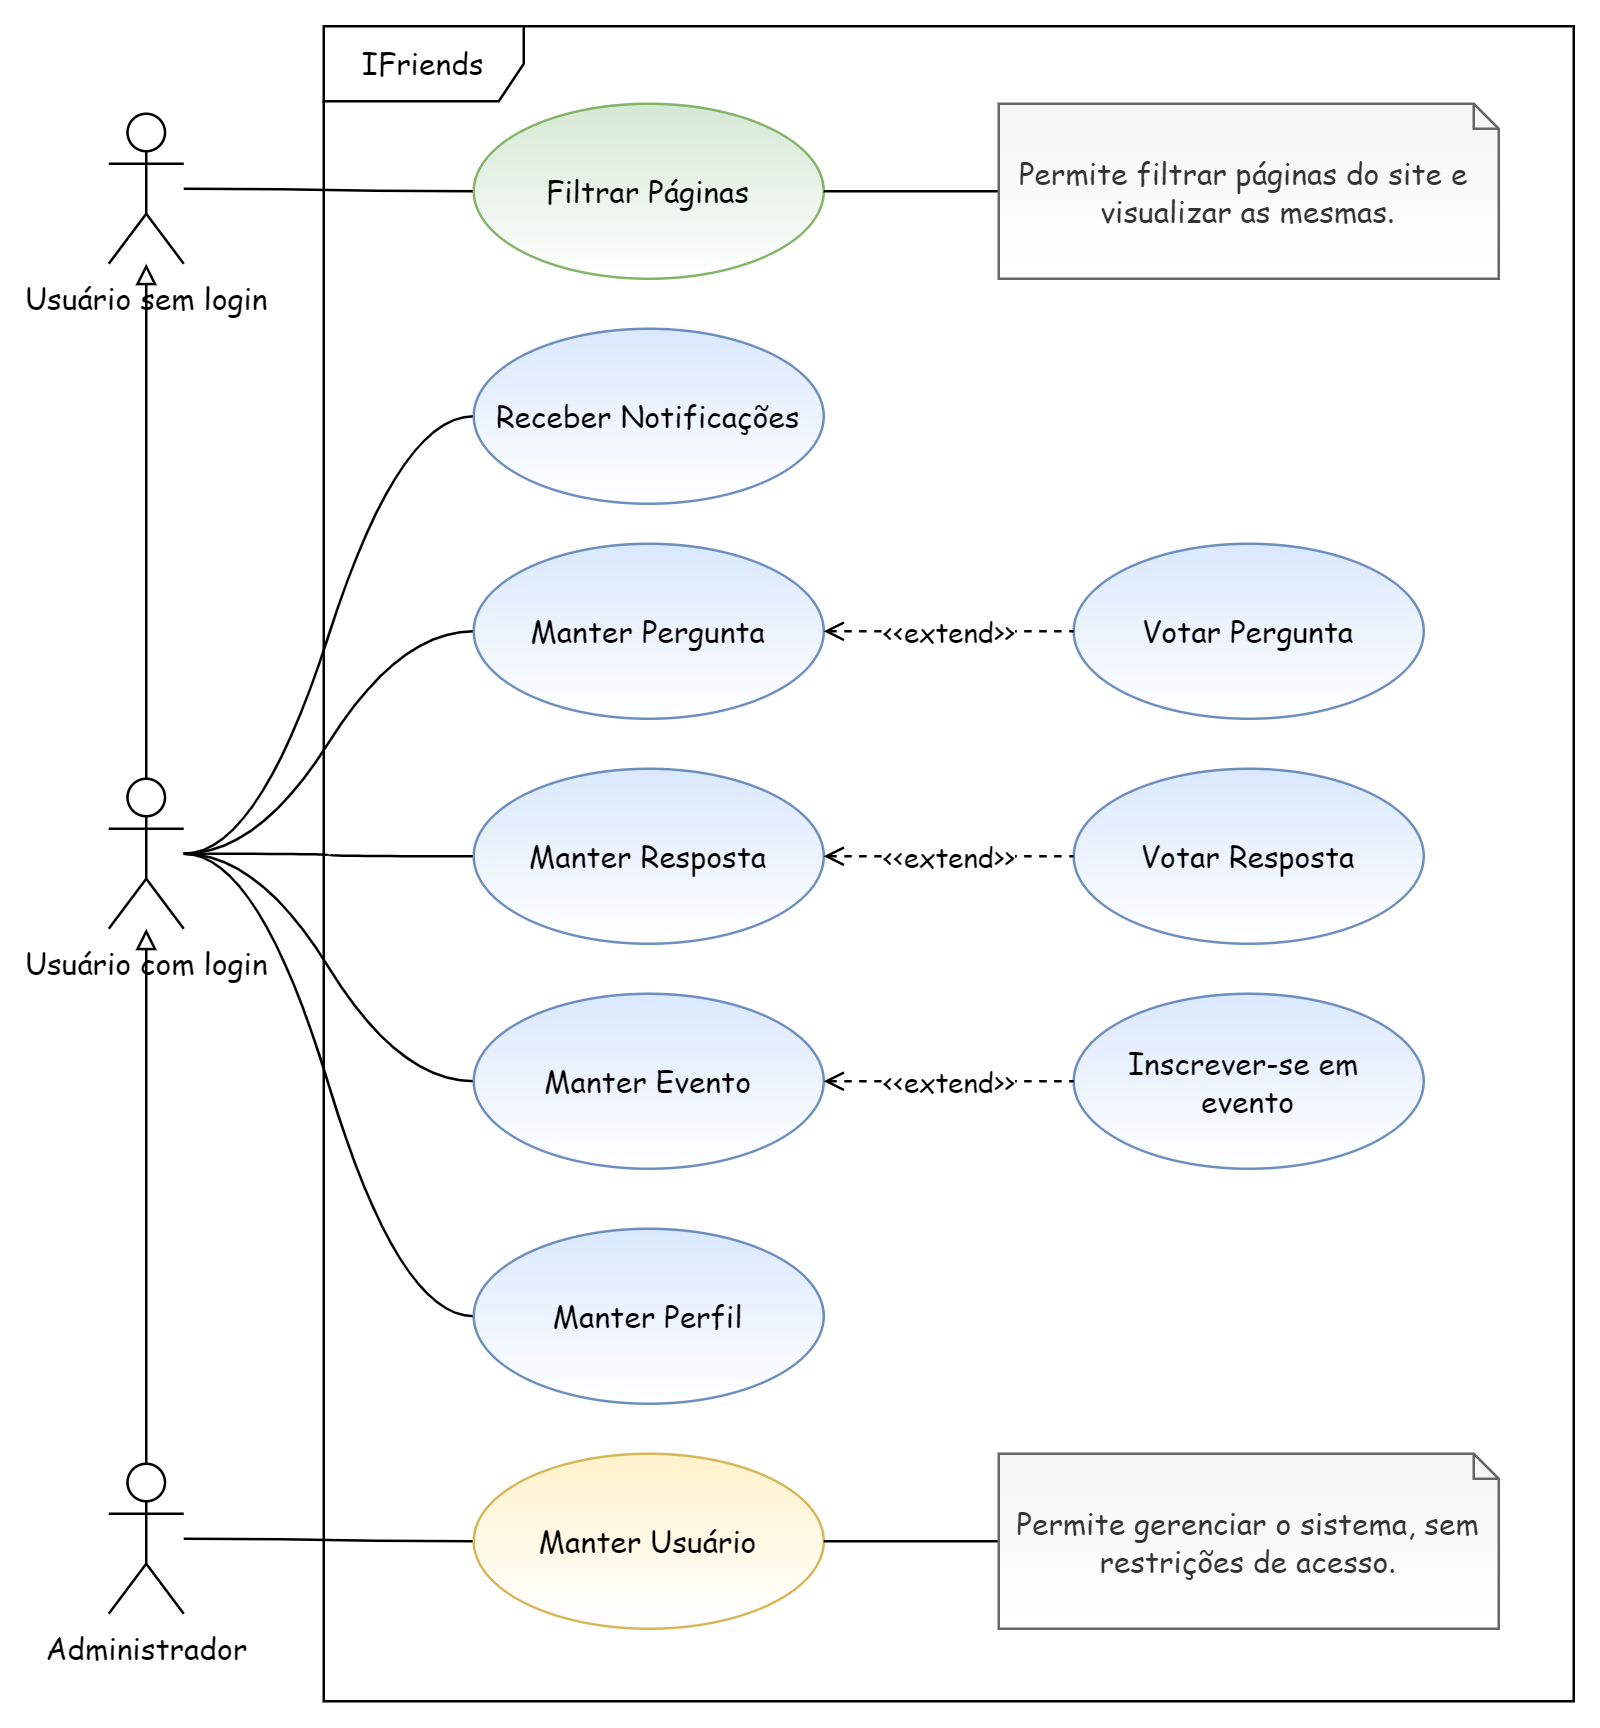
\includegraphics[width=1.0\textwidth]{anexos/Imagens_Diagramas/CasosDeUso_IFriends.png}
\fonte{Os autores.}
\end{figure}
\FloatBarrier


%\subsection{Diagrama de Classes}
% É necessário?

\subsection{Diagrama de Entidade e Relacionamento}

De acordo com \citeonline{leal2015linguagem}, a abordagem entidade-relacionamento é a técnica de modelagem de dados mais difundida e utilizada e representa a modelo conceitual do banco de dados. Nela, a estrutura do banco de dados é descrita como coleção de entidades, relacionamentos e representada graficamente por meio do Diagrama Entidade Relacionamento.

Através dele, é possível descrever um subconjunto do mundo real que será retratado no banco de dados com um alto nível de abstração. Além disso, o modelo Entidade Relacionamento é um modelo formal e caracteriza-se por ter uma grande capacidade semântica, o que garante que todos possam ter o mesmo entendimento \cite{leal2015linguagem}.

A \autoref{diagrama_EntidadeRelacionamento} representa o \ac{der} do projeto de sistema \gls{ifriends}.

\begin{figure}[htb]
\centering
\caption{Diagrama de Entidade e Relacionamento}
\label{diagrama_EntidadeRelacionamento}
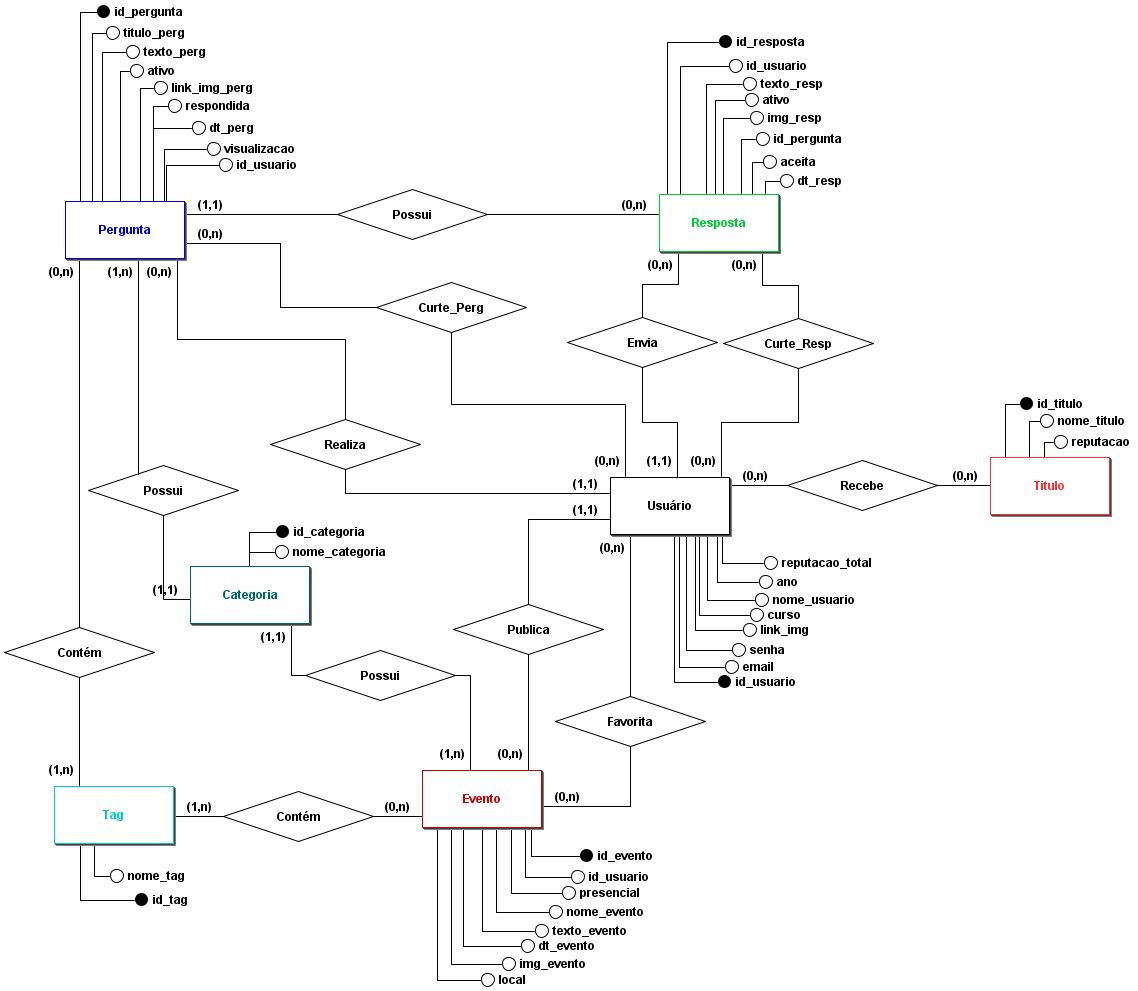
\includegraphics[width=1.0\textwidth]{anexos/Imagens_Diagramas/DER_IFriends.png}
\fonte{Os autores.}
\end{figure}
\FloatBarrier


\subsection{Diagrama de Tabelas Relacionais}

O Diagrama de Tabelas Relacionais \acs{dtr} representa o modelo lógico do Banco de Dados. Segundo \citeonline{utilidadepublica:201?}, através do modelo lógico é representado de maneira mais clara as entidades e os relacionamentos, pois considera algumas limitações e implementa recursos como adequação de padrão e nomenclatura, define as chaves primárias e estrangeiras, normalização, integridade referencial, entre outras.

Deste modo, a \autoref{diagrama_TabelasRelacionais} representa o \ac{dtr} do projeto de sistema \gls{ifriends}.

\begin{figure}[htb]
\centering
\caption{Diagrama de Tabelas Relacionais}
\label{diagrama_TabelasRelacionais}
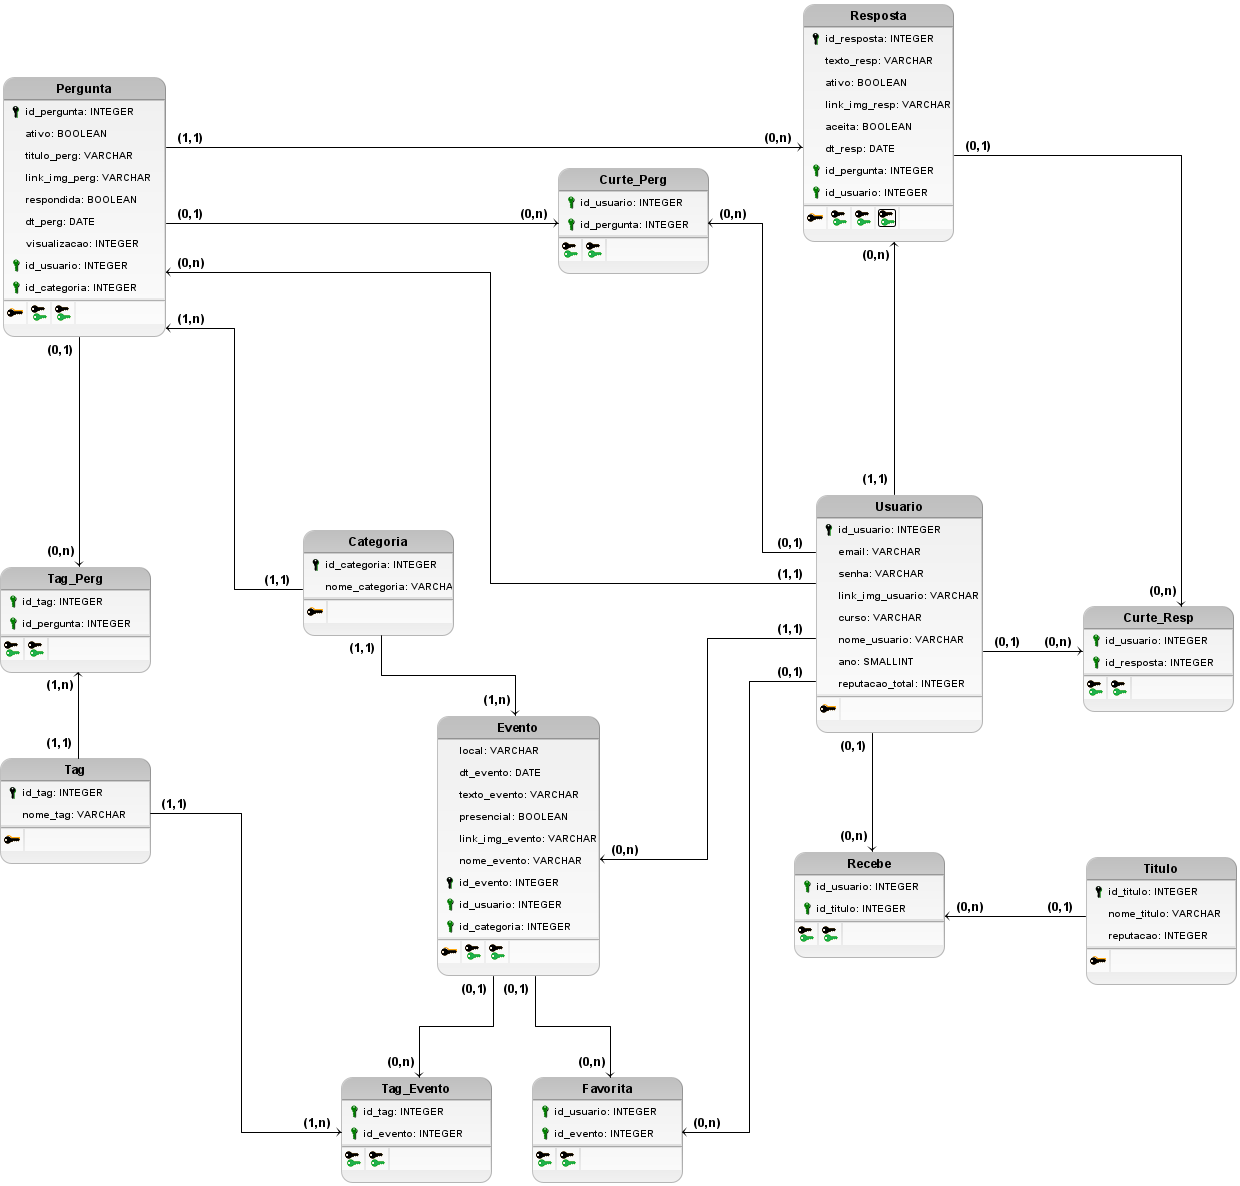
\includegraphics[width=0.9\textwidth]{anexos/Imagens_Diagramas/DTR_IFriends.png}
\fonte{Os autores.}
\end{figure}
\FloatBarrier

\subsection{Dicionário de Dados}

O Dicionário de dados é responsável por armazenar as informações de configuração do banco de dados e as estruturas que compõem suas respectivas tabelas. As estruturas definem os campos e suas propriedades \cite{alvesbanco}.

Conforme \citeonline{date2004introdução}, o Dicionário de dados é o lugar em que – dentre outras coisas – todos os diversos esquemas (externo, conceitual, interno) e todos os mapeamentos correspondentes são mantidos.

O Dicionário de dados contém os metadados, dados que explicam dados, com relação aos diversos objetos que são de interesse do próprio sistema. Exemplos desses objetos incluem índices, usuários, restrições de integridade, restrições de segurança, e assim por diante, informações que essenciais para que o sistema faça seu trabalho apropriadamente \cite{date2004introdução}.

De tal modo, abaixo encontram-se os quadros que representam o \ac{dd} das tabelas de banco de dados do projeto \gls{ifriends}.

%%%%%%%%% Tabela usuario
\def\arraystretch{1.5}

\begin{quadro}[htb]
\centering
\ABNTEXfontereduzida
\caption[Usuário]{Usuário.}
\begin{tabular}{|>{\Centering}m{3cm}|>{\Centering}m{1.75cm}|>{\Centering}m{1.6cm}|>{\Centering}m{1.15cm}|>{\Centering}m{1.25cm}|m{4.5cm}|}
\hline
\thead{Atributo} & \thead{Tipo} & \thead{Tamanho} & \thead{Nulo} & \thead{Chave} & \thead{Descrição}\\
\hline

id\_usuario & INT & 11 & N & PK & Chave primária do usuário \\ \hline
email & VARCHAR & 50 & N &  & E-mail institucional do usuário \\ \hline
senha & VARCHAR & 50 & N &  & Senha de acesso ao sistema \\ \hline
link\_img & TEXT &  & S &  & link da imagem de perfil \\ \hline
curso & VARCHAR & 50 & S &  & Curso atual \\ \hline
nome\_usuario & VARCHAR & 120 & N &  & Nome do usuário \\ \hline
ano & INT & 1 & S &  & Ano que o usuário cursa, ex.: 1\textdegree ano \\ \hline
reputacao\_total & INT & 11 & N  &  & Pontuação da reputação do usuário \\ \hline

\end{tabular}\legend{Fonte: Os autores}
\end{quadro}
\FloatBarrier 

%%%%%%%% Tabela usuario - pergunta
\def\arraystretch{1.5}

\begin{quadro}[htb]
\centering
\ABNTEXfontereduzida
\caption[Usuário\_Pergunta]{Usuário\_Pergunta.}
\label{quadro-dicionario-dados}
\begin{tabular}{|>{\Centering}m{3cm}|>{\Centering}m{1.75cm}|>{\Centering}m{1.6cm}|>{\Centering}m{1.15cm}|>{\Centering}m{1.25cm}|m{4.5cm}|}
\hline
\thead{Atributo} & \thead{Tipo} & \thead{Tamanho} & \thead{Nulo} & \thead{Chave} & \thead{Descrição}\\
\hline

id\_usuario & INT & 11 & N & FK & Chave estrangeira no usuário \\ \hline
id\_pergunta & INT & 11 & N & FK & Chave estrangeira na pergunta \\ \hline

\end{tabular}\legend{Fonte: Os autores}
\end{quadro}
\FloatBarrier 

%\clearpage

%usuario - resposta
\def\arraystretch{1.5}

\begin{quadro}[htb]
\centering
\ABNTEXfontereduzida
\caption[Usuário\_Resposta]{Usuário\_Resposta.}
\label{quadro-dicionario-dados}
\begin{tabular}{|>{\Centering}m{3cm}|>{\Centering}m{1.75cm}|>{\Centering}m{1.6cm}|>{\Centering}m{1.15cm}|>{\Centering}m{1.25cm}|m{4.5cm}|}
\hline
\thead{Atributo} & \thead{Tipo} & \thead{Tamanho} & \thead{Nulo} & \thead{Chave} & \thead{Descrição}\\
\hline

id\_usuario & INT & 11 & N & FK & Chave estrangeira no usuário \\ \hline
id\_resposta & INT & 11 & N & FK & Chave estrangeira na resposta \\ \hline

\end{tabular}\legend{Fonte: Os autores}
\end{quadro}
\FloatBarrier 

%usuario - Titulo
\def\arraystretch{1.5}

\begin{quadro}[htb]
\centering
\ABNTEXfontereduzida
\caption[Usuário\_Título]{Usuário\_Título.}
\label{quadro-dicionario-dados}
\begin{tabular}{|>{\Centering}m{3cm}|>{\Centering}m{1.75cm}|>{\Centering}m{1.6cm}|>{\Centering}m{1.15cm}|>{\Centering}m{1.25cm}|m{4.5cm}|}
\hline
\thead{Atributo} & \thead{Tipo} & \thead{Tamanho} & \thead{Nulo} & \thead{Chave} & \thead{Descrição}\\
\hline

id\_usuario & INT & 11 & N & FK & Chave estrangeira no usuário \\ \hline
id\_titulo & INT & 11 & N & FK & Chave estrangeira no titulo \\ \hline

\end{tabular}\legend{Fonte: Os autores}
\end{quadro}
\FloatBarrier 


%Titulo
\def\arraystretch{1.5}

\begin{quadro}[htb]
\centering
\ABNTEXfontereduzida
\caption[Título]{Título.}
\label{quadro-dicionario-dados}
\begin{tabular}{|>{\Centering}m{3cm}|>{\Centering}m{1.75cm}|>{\Centering}m{1.6cm}|>{\Centering}m{1.15cm}|>{\Centering}m{1.25cm}|m{4.5cm}|}
\hline
\thead{Atributo} & \thead{Tipo} & \thead{Tamanho} & \thead{Nulo} & \thead{Chave} & \thead{Descrição}\\
\hline

id\_titulo & INT & 11 & N & PK & Chave primária do título \\ \hline
nome\_titulo & VARCHAR & 50 & N &  & Nome do título \\ \hline
reputacao & INT & 11 & N & & Acumulo da pontuação \\\hline

\end{tabular}\legend{Fonte: Os autores}
\end{quadro}
\FloatBarrier 
%\clearpage

%Resposta
\def\arraystretch{1.5}

\begin{quadro}[htb]
\centering
\ABNTEXfontereduzida
\caption[Resposta]{Resposta.}
\label{quadro-dicionario-dados}
\begin{tabular}{|>{\Centering}m{3cm}|>{\Centering}m{1.75cm}|>{\Centering}m{1.6cm}|>{\Centering}m{1.15cm}|>{\Centering}m{1.25cm}|m{4.5cm}|}
\hline
\thead{Atributo} & \thead{Tipo} & \thead{Tamanho} & \thead{Nulo} & \thead{Chave} & \thead{Descrição}\\ \hline

id\_resposta & INT & 11 & N & PK & Chave primária da resposta \\ \hline
id\_usuario & INT & 11 & N & FK  & Chave estrangeira de usuário \\ \hline
id\_pergunta & INT & 11 & N & FK & Chave estrangeira de pergunta \\ \hline
texto\_resp & TEXT &  & N &  & Conteúdo da resposta \\ \hline
ativo & BOOLEAN & & N & & Resposta ativa ou não \\ \hline
img\_resp & TEXT & & S & & Imagem da resposta \\ \hline
aceita & BOOLEAN & & N & & Se a resposta foi aceita como solução válida para o autor da pergunta \\ \hline
dt\_resposta & DATE & 50 & N & & Data em que a resposta foi publicada \\ \hline

\end{tabular}\legend{Fonte: Os autores}
\end{quadro}
\FloatBarrier 

%Tag
\def\arraystretch{1.5}

\begin{quadro}[htb]
\centering
\ABNTEXfontereduzida
\caption[Tag]{Tag.}
\label{quadro-dicionario-dados}
\begin{tabular}{|>{\Centering}m{3cm}|>{\Centering}m{1.75cm}|>{\Centering}m{1.6cm}|>{\Centering}m{1.15cm}|>{\Centering}m{1.25cm}|m{4.5cm}|}
\hline
\thead{Atributo} & \thead{Tipo} & \thead{Tamanho} & \thead{Nulo} & \thead{Chave} & \thead{Descrição}\\
\hline

id\_tag & INT & 3 & N & PK & Chave primária da tag \\ \hline
nome\_tag & VARCHAR & 50 & N &  & Nome da tag \\ \hline

\end{tabular}\legend{Fonte: Os autores}
\end{quadro}
\FloatBarrier 
%\clearpage

%Pergunta
\def\arraystretch{1.5}

\begin{quadro}[htb]
\centering
\ABNTEXfontereduzida
\caption[Pergunta]{Pergunta.}
\label{quadro-dicionario-dados}
\begin{tabular}{|>{\Centering}m{3cm}|>{\Centering}m{1.75cm}|>{\Centering}m{1.6cm}|>{\Centering}m{1.15cm}|>{\Centering}m{1.25cm}|m{4.5cm}|}
\hline
\thead{Atributo} & \thead{Tipo} & \thead{Tamanho} & \thead{Nulo} & \thead{Chave} & \thead{Descrição}\\ \hline

id\_pergunta & INT & 11 & N & PK & Chave primária da pergunta \\ \hline
id\_usuario & INT & 11 & N & FK  & Chave estrangeira de usuário \\ \hline
dt\_perg & DATE &  & N & & Data da pergunta \\ \hline
titulo\_perg & VARCHAR & 50 & N & & Título da pergunta \\ \hline
texto\_perg & TEXT & & N & & Descrição da pergunta \\ \hline
ativo & BOOLEAN & & N & & Pergunta ativa ou não \\ \hline
link\_img\_perg & TEXT & & S & & Link da imagem da pergunta \\ \hline
respondida & BOOLEAN & & N & & Se a pergunta já teve uma resposta útil a quem perguntou \\ \hline
visualizações & INT & 5 & N & & Quantidade de visualizações da pergunta \\ \hline

\end{tabular}\legend{Fonte: Os autores}
\end{quadro}
\FloatBarrier 


%Tag - Pergunta
\def\arraystretch{1.5}

\begin{quadro}[htb]
\centering
\ABNTEXfontereduzida
\caption[Tag\_Pergunta]{Tag\_Pergunta.}
\label{quadro-dicionario-dados}
\begin{tabular}{|>{\Centering}m{3cm}|>{\Centering}m{1.75cm}|>{\Centering}m{1.6cm}|>{\Centering}m{1.15cm}|>{\Centering}m{1.25cm}|m{4.5cm}|}
\hline
\thead{Atributo} & \thead{Tipo} & \thead{Tamanho} & \thead{Nulo} & \thead{Chave} & \thead{Descrição}\\ \hline

id\_assunto & INT & 11 & N & FK & Chave estrangeira no assunto \\ \hline
id\_pergunta & INT & 11 & N & FK & Chave estrangeira na pergunta \\ \hline

\end{tabular}\legend{Fonte: Os autores}
\end{quadro}
\FloatBarrier 
%\clearpage

%Tag - Evento
\def\arraystretch{1.5}

\begin{quadro}[htb]
\centering
\ABNTEXfontereduzida
\caption[Tag\_Evento]{Tag\_Evento.}
\label{quadro-dicionario-dados}
\begin{tabular}{|>{\Centering}m{3cm}|>{\Centering}m{1.75cm}|>{\Centering}m{1.6cm}|>{\Centering}m{1.15cm}|>{\Centering}m{1.25cm}|m{4.5cm}|}
\hline
\thead{Atributo} & \thead{Tipo} & \thead{Tamanho} & \thead{Nulo} & \thead{Chave} & \thead{Descrição}\\ \hline

id\_assunto & INT & 11 & N & FK & Chave estrangeira no assunto \\ \hline
id\_evento & INT & 11 & N & FK & Chave estrangeira no evento \\ \hline

\end{tabular}\legend{Fonte: Os autores}
\end{quadro}
\FloatBarrier 

%evento
\def\arraystretch{1.5}

\begin{quadro}[htb]
\centering
\ABNTEXfontereduzida
\caption[Evento]{Evento.}
\label{quadro-dicionario-dados}
\begin{tabular}{|>{\Centering}m{3cm}|>{\Centering}m{1.75cm}|>{\Centering}m{1.6cm}|>{\Centering}m{1.15cm}|>{\Centering}m{1.25cm}|m{4.5cm}|}
\hline
\thead{Atributo} & \thead{Tipo} & \thead{Tamanho} & \thead{Nulo} & \thead{Chave} & \thead{Descrição}\\
\hline

id\_evento & INT & 11 & N & PK & Chave primária do evento \\ \hline
id\_usuario & INT & 11 & S & FK  & Chave estrangeira de usuário \\ \hline
presencial & char & 1 & N & & Local do evento, sendo presencial, online ou ambos \\ \hline
nome\_evento & VARCHAR & 50 & N & & Nome do evento \\ \hline
texto\_evento & TEXT &  & N & & Descrição sobre o evento \\ \hline
dt\_evento & DATE & & N & & Data que o evento ocorrerá \\ \hline
img\_evento & TEXT &  & S & & Imagem do evento \\ \hline
local & TEXT & & N & & Local onde será realizado, tanto presencial como online \\ \hline
\end{tabular}\legend{Fonte: Os autores}
\end{quadro}
\FloatBarrier 

%Categoria
\def\arraystretch{1.5}

\begin{quadro}[htb]
\centering
\ABNTEXfontereduzida
\caption[Categoria]{Categoria.}
\label{quadro-dicionario-dados}
\begin{tabular}{|>{\Centering}m{3cm}|>{\Centering}m{1.75cm}|>{\Centering}m{1.6cm}|>{\Centering}m{1.15cm}|>{\Centering}m{1.25cm}|m{4.5cm}|}
\hline
\thead{Atributo} & \thead{Tipo} & \thead{Tamanho} & \thead{Nulo} & \thead{Chave} & \thead{Descrição}\\
\hline

id\_categoria & INT & 11 & N & PK & Chave primária da categoria \\ \hline
nome\_categoria & INT & 50 & N & FK & Nome da categoria \\ \hline

\end{tabular}\legend{Fonte: Os autores}
\end{quadro}
\FloatBarrier 

%\clearpage

\section{Prototipagem}
Segundo \citeonline{ferreira:2020}, ``prototipar é trazer, para o mundo real, o mundo palpável, as ideias de negócio construídas no mundo abstrato, na teoria''. Isto é, o autor comenta que um protótipo é um recurso utilizado para demonstrar e escolher a solução para representar uma ideia, podendo ser efetuado com entregas digitais, como telas de sistema. Dado isto, a próxima seção apresentará as telas prototipadas do projeto de sistema \gls{ifriends}.

Ainda, para auxiliar na prototipação das telas, foi elaborado um mapa mental de modo a representar melhor o fluxo do nosso projeto, que pode ser conferido na \autoref{Mapa mental}.

\begin{figure}[htb]
\centering
\caption{\label{Mapa mental} Mapa mental}
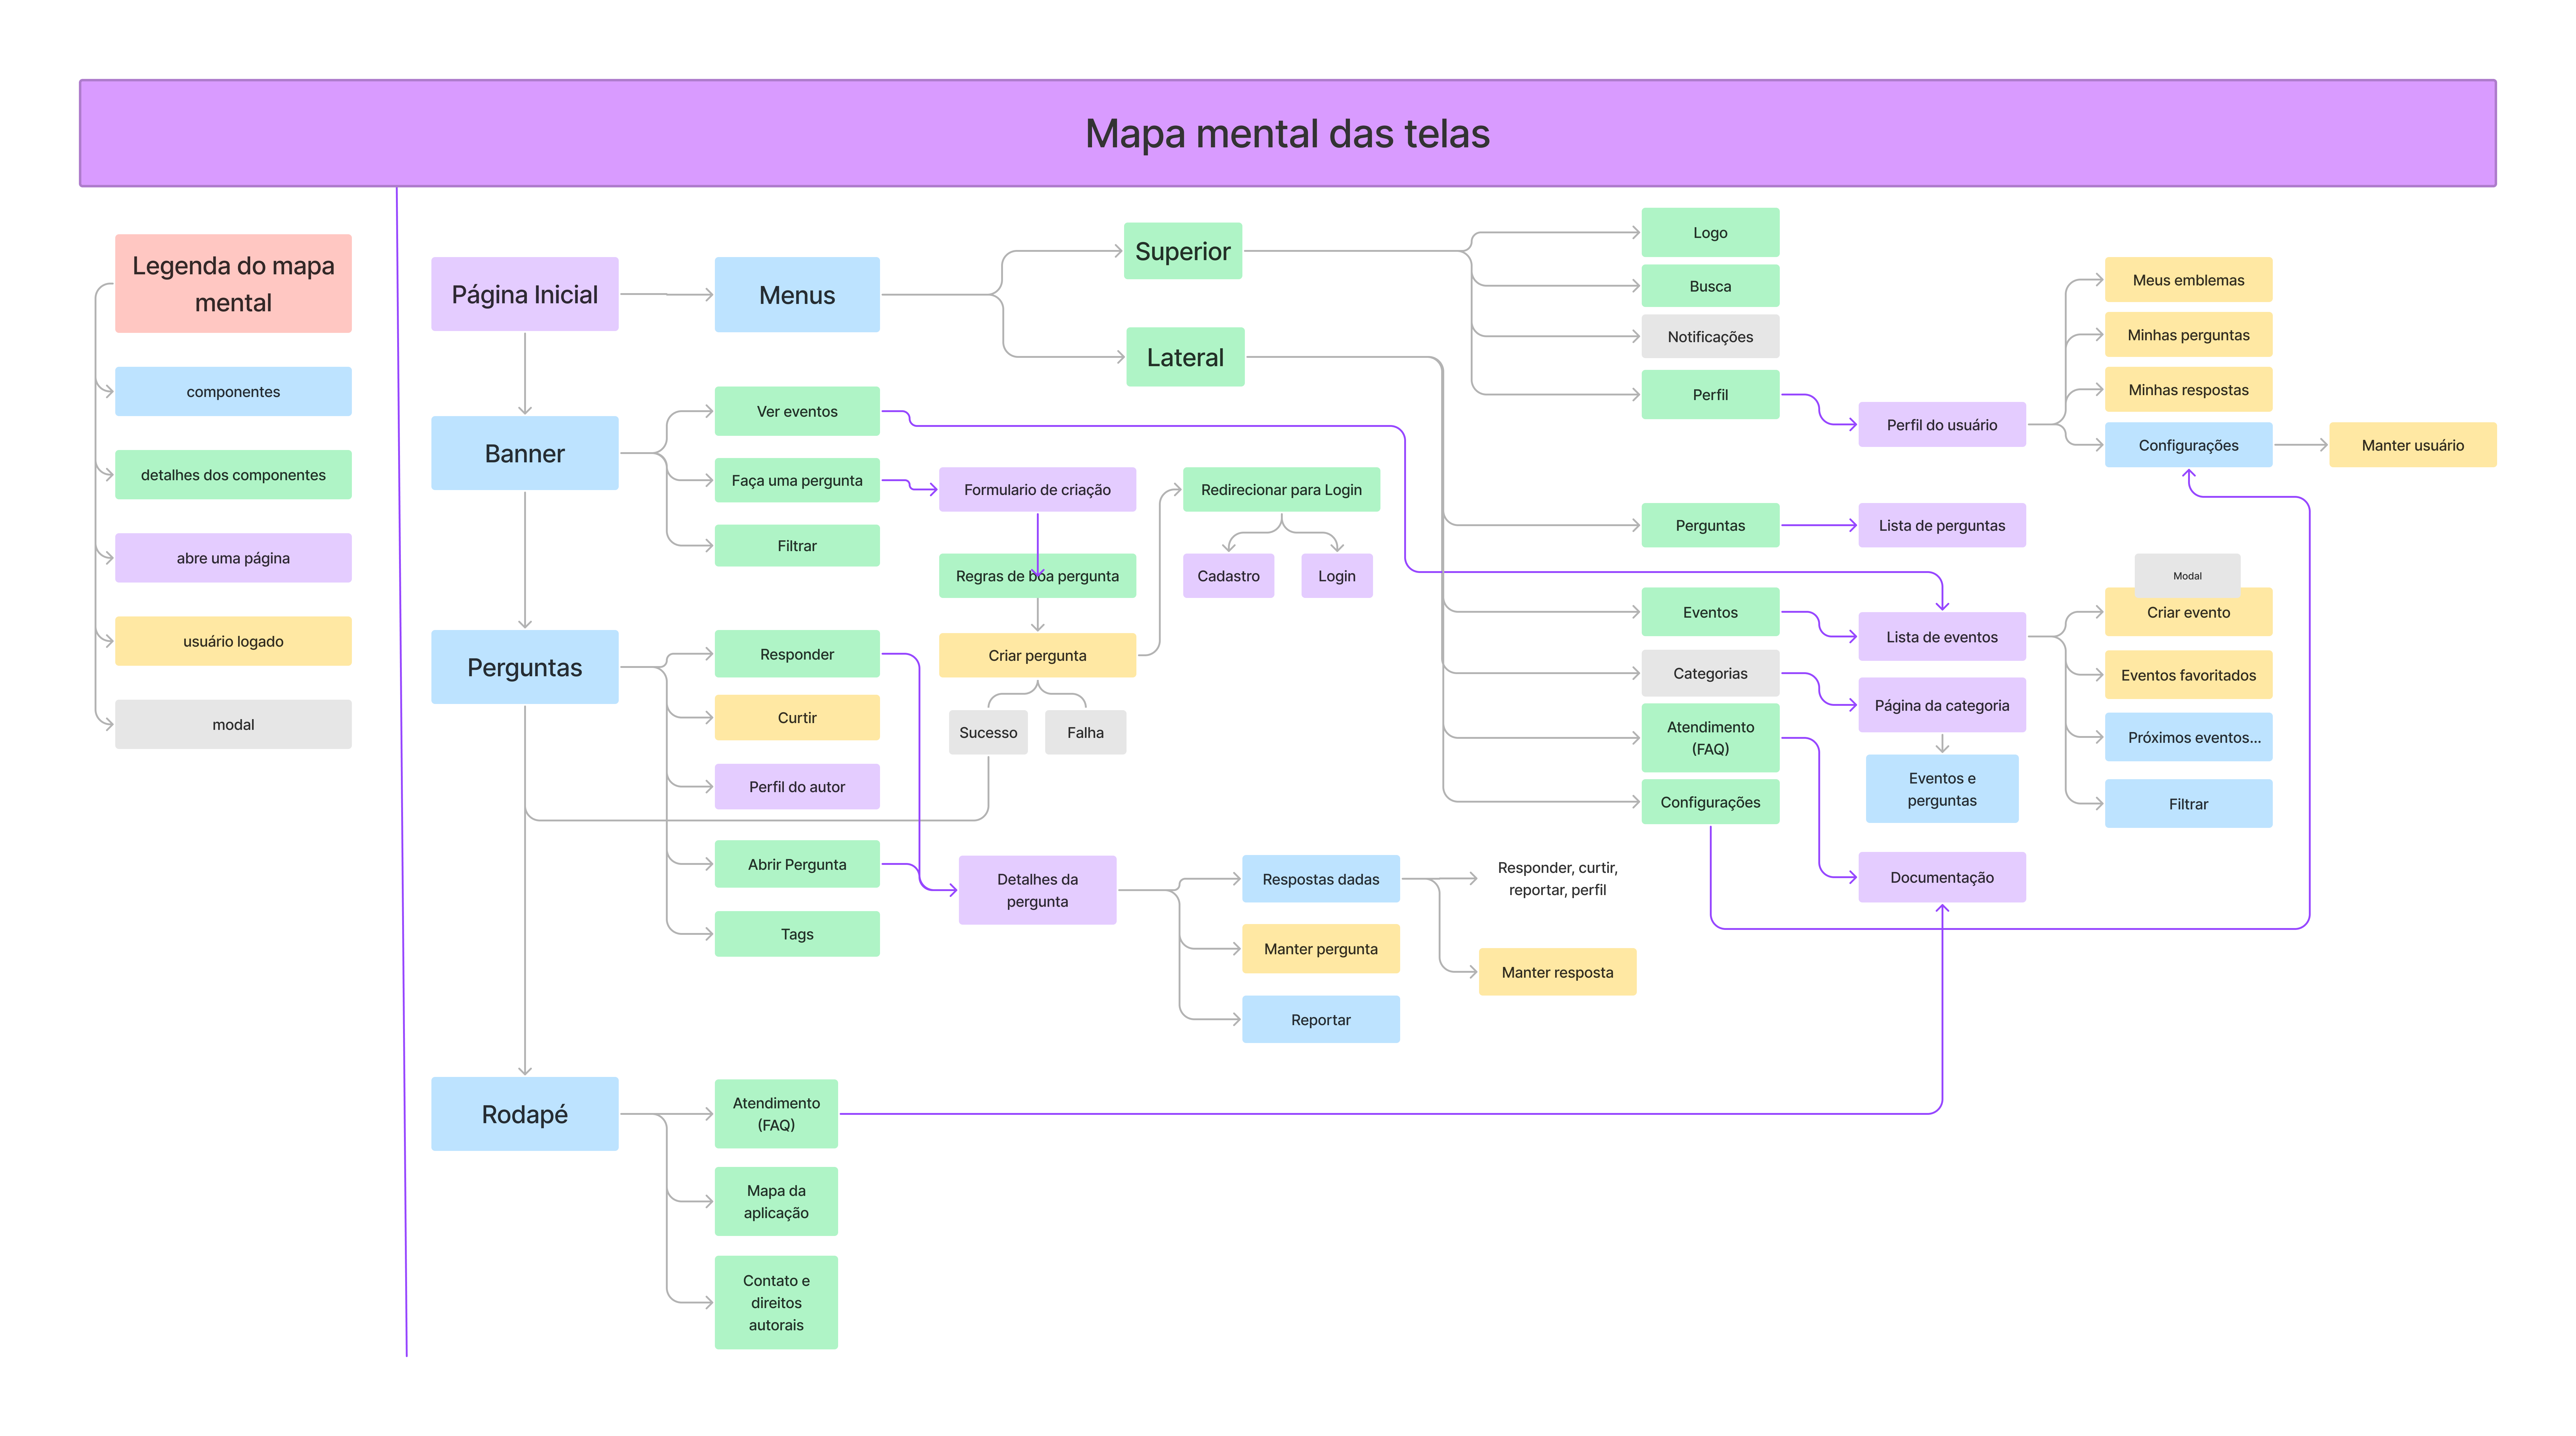
\includegraphics[width=1\textwidth]{anexos/Imagens_Prototipo/Mapa_Mental.png}
\fonte{os autores}
\end{figure}
\FloatBarrier

\subsection{Protótipos de alta fidelidade}
Nesta seção estão contidas as figuras que representam as principais telas do sistema em relação a \gls{POC} do projeto, cada tela apresenta uma breve contextualização sobre o seu conteúdo. De todo modo, a apresentação pode ser visualizada também pelo \href{https://www.figma.com/proto/GhIlybDubGmr3NkRU0a9GP/Protótipo---IFriends?node-id=73\%3A321}{Figma}.

A \autoref{Home Page} apresenta a página inicial do projeto, onde o usuário entra em contato pela primeira vez com o sistema. Nela o usuário pode navegar através de dois menus disponíveis na página: o lateral e o superior, usar a barra de pesquisa, \textit{logar} no seu perfil, acessar as suas configurações, entre outras ações disponibilizadas. Na página encontram as questões mais relevantes da comunidade, assim como os espaços destinados para a realização de uma pergunta ou de uma monitoria.

\begin{figure}[htb]
\centering
\caption{\label{Home Page} Página inicial}
\includesvg[inkscapelatex=false,width=0.7\textwidth]{anexos/Imagens_Prototipo/Home_Page.svg}
\fonte{os autores}
\end{figure}
\FloatBarrier

Quando o usuário clica em uma pergunta ou em ``Responder'' ele é direcionado à página dessa pergunta como mostra a \autoref{Pergunta e respostas}, nela ele pode encontrar as respostas já fornecidas por outros membros da comunidade, assim como também pode deixar a sua contribuição.

\begin{figure}[htb]
\centering
\caption{\label{Pergunta e respostas} Pergunta e respostas}
\includesvg[inkscapelatex=false,width=0.9\textwidth]{anexos/Imagens_Prototipo/Pergunta_Respostas.svg}
\fonte{os autores}
\end{figure}
\FloatBarrier

Já a \autoref{Cadastro de perguntas} corresponde a página de cadastro de perguntas, nessa tela são apresentados todos os elementos julgados necessários para a sua realização, nesta página ainda de encontra o manual de uma boa pergunta, tal foi elaborado com o intuito de ajudar e auxiliar o usuário na preparação de sua problemática. 

\begin{figure}[htb]
\centering
\caption{\label{Cadastro de perguntas} Cadastro de perguntas}
\includesvg[inkscapelatex=false,width=0.9\textwidth]{anexos/Imagens_Prototipo/Cadastro_Perguntas.svg}
\fonte{os autores}
\end{figure}
\FloatBarrier

As telas apresentadas até o momento são aquelas que se encontram relacionadas com a \gls{POC}, portanto vale salientar que esta seção será atualizada futuramente conforme o andamento e elaboração do projeto.


%---------------------------------------------------------------------------------------






% ---
% Conclusão (outro exemplo de capítulo sem numeração e presente no sumário)
% Dependendo do trabalho desenvolvido ele pode ter uma Conclusão ou Considerações finais
% Para trabalhos de disciplina utilizar Considerações Finais

\chapter{Prova de Conceito}

De acordo com \citeonline {lima2020usando}, prova de conceito ou \acs{POC} é o nome que se dá à demonstração da probabilidade de validação de uma ideia (ou conceito), podendo ser na área de TI ou na área dos negócios. A \acs{POC} pode ser aplicada em um protótipo ou em um projeto em fase inicial, e normalmente segue um roteiro de testes. Esses testes são evidências, que demonstram que um conceito de design, proposta de negócio entre outros, são viáveis.

Segundo \citeonline {lima2020usando}, só é necessário realizar a prova de conceito, sempre que há desejo de implementar mudanças relacionadas a processos, ferramentas ou métodos, e isso se dá através dos testes designados pela mesma. Através da \acs{POC} é possível determinar se o serviço ou produto funciona na prática e qual seu respectivo nível de eficácia e eficiência, além de ser extremamente importante tanto para o cliente como para o desenvolvedor, que no que lhe concerne, adquire a chance de implementar uma solução em um ambiente real de mercado onde todas as variáveis e possibilidades que podem acabar influenciando na solução, são expostas.

Para a prova de conceito do projeto de sistema \gls{ifriends}, escolheu-se desenvolver, considerando a utilização do método ágil, apenas dois \textit{Épicos}: Gestão de Perguntas e Gestão de Respostas, descritos na seção de análise de requisitos. Isto, pois, após discussões em equipe e analisando a definição de \acs{POC}, os integrantes chegaram a um consenso de que estes são os itens mais fundamentais para que o funcionamento do projeto seja provado. 

Utilizando as tecnologias elencadas anteriormente, foi possível criar todas as requisições escolhidas nos épicos para a \acs{api} do projeto, e ainda pode-se publicá-la no \gls{heroku}, disponível na \autoref{qrcode_api} e conseguimos chamá-la no \textit{front-end} da aplicação através da biblioteca Axios.

\begin{figure}[htb]
\centering
\caption{\href{https://ifriends-api.herokuapp.com/}{API IFriends}}

\label{qrcode_api}
\qrcode{https://ifriends-api.herokuapp.com/}
\fonte{Os autores}
\end{figure}
\FloatBarrier

 No entanto, ao publicar a aplicação ReactJS no \gls{heroku}, disponível na \autoref{qrcode_app-ifriends}, foi gerado um erro de limite de memória do Node.JS excedido, e portanto, aplicação saiu do ar. Isto ocorreu após terem sido adicionados mais recursos nela, ou seja, no último \textsl{deploy} feito. Outro ponto é que este problema acontece somente após serem feitas algumas requisições, e não no momento em que é feito o \textsl{deploy} e mesmo aumentando a capacidade miníma de memória, o erro persistiu. A equipe pretende assim investigar o fato ocorrido para tomar possíveis planos de ação para as melhorias no projeto, partindo inicialmente da \href{https://devcenter.heroku.com/articles/node-memory-use}{documentação do \gls{heroku}}, que visa explicar o problema e trazer mais possíveis soluções.
 
\begin{figure}[htb]
\centering
\caption{\href{https://app-ifriends.herokuapp.com}{Aplicação IFriends}}
\label{qrcode_app-ifriends}
\qrcode{https://app-ifriends.herokuapp.com}
\fonte{Os autores}
\end{figure}
\FloatBarrier

Com relação aos demais fatores do sistema, a equipe notou que foi possível testar a solução de maneira satisfatória, ainda que alguns problemas tenham acontecido no meio do caminho. A respeito da internacionalização e da criptografia, por exemplo, conseguiu-se encontrar recursos para fazê-las, visto que, no ReactJS, podemos definir a internacionalização com a biblioteca \href{https://ant.design/components/config-provider/}{Ant Design}, porém a solução apresentou instabilidade após a implementação, e dessa forma, optou-se por não demonstrá-la na apresentação. Além disso, foi percebido que o próprio \gls{heroku} disponibiliza meios para inclusão da criptografia do sistema, mas conforme dito anteriormente, precisa-se solucionar o problema da hospedagem para que todos os recursos do sistema estejam funcionando on-line de maneira correta.

Dentre as demais mudanças feitas no projeto está a utilização do \textsl{Scoold} apenas como referência para o desenvolvimento, e não mais como uma tecnologia a ser incorporada no sistema. 

Por outro lado, espera-se que após todos os apontamentos feitos, o projeto possa ser melhorado de forma iterativa para que a entrega da primeira versão seja feita sem instabilidades e, além disso, que a equipe possa realizar as entregas nos devidos prazos e com o cumprimento de todos os requisitos propostos.


% \chapter{Considerações finais}
% Esta seção será preenchida futuramente, após o desenvolvimento das demais partes do projeto.

% ----------------------------------------------------------
% Finaliza a parte no bookmark do PDF
% para que se inicie o bookmark na raiz
% e adiciona espaço de parte no Sumário
% ----------------------------------------------------------
\phantompart

% ----------------------------------------------------------
% ELEMENTOS PÓS-TEXTUAIS
% ----------------------------------------------------------
\postextual
% ----------------------------------------------------------
% ----------------------------------------------------------
% Referências bibliográficas
% ----------------------------------------------------------

\bibliography{referencias,exemplos/abntex2-doc-abnt-6023}

% ----------------------------------------------------------
% Glossário
% ----------------------------------------------------------
%
%
\ifdef{\printnoidxglossary}{
    \addcontentsline{toc}{chapter}{GLOSSÁRIO}
    \printnoidxglossary[style=glossario]
    %\printglossaries
    % \cleardoublepage
}{
}

% ----------------------------------------------------------
% Apêndices
% Documentos gerados pelo próprio autor
% ----------------------------------------------------------

% ---
% Inicia os apêndices
% ---
\begin{apendicesenv}

% Imprime uma página indicando o início dos apêndices
\partapendices

% ----------------------------------------------------------
\chapter{Perguntas da pesquisa de viabilidade}
\label{questões}
% ----------------------------------------------------------
\begin{enumerate}
  \item Qual é o seu grau de escolaridade?
  \item Qual é o seu curso?
  \item Você trabalha ou faz estágio?
  \item Você sentiu dificuldade em se adaptar ao entrar no IF?
  \item Descreva como foi a sua experiência (com relação as dificuldades na instituição e no ensino).
  \item Com que frequência você costuma ir às monitorias?
  \item Você usaria um sistema de perguntas e respostas do IF?
  \item Você acredita que uma comunidade de perguntas e respostas te ajudaria na sua vida acadêmica?
  \item De que forma isso faria/não faria diferença para você? (Fique a vontade de responder com toda sinceridade!).
  \item Gostaria de compartilhar mais alguma coisa sobre o tema? Bem, sinta-se a vontade!
\end{enumerate}
\chapter{Atas das Reuniões}

\label{atasReunioes}
\section{1\textordmasculine bimestre}
\subsection{Planejamento - 15/03/2022}
\noindent Integrantes: Anaí Rojas, Jamilli Gioielli, José Roberto, Julia Romualdo, Kaiky Matsumoto. \\
Local: \gls{discord}. \\
Pauta(s): Primeira reunião realizada pela equipe com o objetivo de planejar os passos iniciais do projeto, nela a equipe estabeleceu um contrato social na plataforma \gls{figma} contendo os combinados essenciais para o convívio social entre os componentes da equipe e também iniciou-se um \textsl{board} de ideias iniciais para o projeto.

\subsection{Planejamento/Alinhamento - 17/03/2022}
\noindent Integrantes: Anaí Rojas, Jamilli Gioielli, José Roberto, Julia Romualdo, Kaiky Matsumoto. \\
Local: \gls{discord}.\\
Pauta(s): Reunião de planejamento e alinhamento, onde o foco da equipe esteve em discutir as ideias pré-selecionadas na reunião anterior para o projeto. Desde este primeiro momento a atenção da equipe se voltava principalmente para uma comunidade de dúvidas entre os estudantes do IF. \\
Para organização das tarefas e da equipe a plataforma \gls{notion}, onde o quadro de \textsl{kanban} se encontra, foi criado e organizado inicialmente. \\
A equipe decidiu inicialmente que realizará reuniões nos dias e horários das janelas entre as aulas, permitidas pela grade curricular.

\subsection{Planejamento/Alinhamento - 18/03/2022}
\noindent Integrantes: Anaí Rojas, Jamilli Gioielli, José Roberto, Julia Romualdo, Kaiky Matsumoto. \\
Local: \gls{discord}.\\
Pauta(s): Reunião de planejamento onde a equipe discutiu as tarefas a serem realizadas e discutiu outras ferramentas de organização. \\
Criamos o canal do \gls{youtube}.\\
Realizamos a primeira postagem para o \textsl{blog} da equipe.\\
Amadurecemos ainda mais a ideia da comunidade, pensando em mais funcionalidades para agregar na aplicação e anotando as dúvidas a respeito do tema e do funcionamento.

\subsection{Alinhamento - 21/03/2022}
\noindent Integrantes: Anaí Rojas, Jamilli Gioielli, José Roberto, Julia Romualdo, Kaiky Matsumoto. \\
Local: Saguão \acs{ifsp}.\\
Pauta(s): Reunião realizada antes da aula de \acs{pds} para a equipe discutir algumas dúvidas, perspectivas e ideias sobre o projeto, visando otimizar o tempo em sala de aula.

\subsection{Alinhamento - 25/03/2022}
\noindent Integrantes: Anaí Rojas, Jamilli Gioielli, José Roberto, Julia Romualdo, Kaiky Matsumoto. \\
Local: \gls{discord}.\\
Pauta(s): Reunião de alinhamento, onde a equipe pesquisou em trabalhos anteriores a formatação do documento da proposta inicial para preparar as etapas. 
Aproveitamos também para melhorar o \textsl{layout} do \textsl{blog} da equipe.

\subsection{Planejamento/Alinhamento - 28/03/2022}
\noindent Integrantes: Anaí Rojas, Jamilli Gioielli, José Roberto, Julia Romualdo, Kaiky Matsumoto. \\
Local: Laboratório \acs{ifsp}.\\
Pauta(s): Reunião de alinhamento e planejamento, onde a equipe conversou com os orientadores sobre soluções e funcionalidades para a proposta da comunidade. Neste ponto, resolvemos um problema antigo, validar que o usuário seja de fato aluno da instituição, a solução encontrada foi enviar um \textsl{e-mail} de validação para o \textsl{e-mail} institucional do aluno. Foi citado também outra proposta de projeto para a equipe realizar, uma plataforma de controle e gestão financeira. Porém, a equipe optou por seguir na proposta da comunidade.\\
Partimos para as tarefas, iniciando o desenvolvimento de um questionário direcionado aos alunos do instituto para estudar a viabilidade de criação do projeto.\\
Sobre o \textsl{blog}, finalizamos a melhoria de seu \textsl{layout} e definimos que as publicações serão realizadas aos sábados pela manhã.

\subsection{Planejamento/Retrospectiva - 02/04/2022}
\noindent Integrantes: Anaí Rojas, Jamilli Gioielli, José Roberto, Julia Romualdo, Kaiky Matsumoto. \\
Local: \gls{discord}.\\
Pauta(s): Reunião de retrospectiva e planejamento das atividades, onde revisamos a publicação da semana no \textsl{blog} e as perguntas para a pesquisa de viabilidade. Realizamos a entrega sobre as tecnologias que serão utilizadas no desenvolvimento do projeto no \gls{moodle} da disciplina e definimos duas tarefas: divulgação da pesquisa de viabilidade a partir de segunda-feira para alunos e ex-alunos da instituição e gerenciamento do \textsl{backlog} para cada parte do projeto.

\subsection{Planejamento - 04/04/2022}
\noindent Integrantes: Anaí Rojas, Jamilli Gioielli, José Roberto, Julia Romualdo, Kaiky Matsumoto. \\
Local: Laboratório \acs{ifsp}.\\
Pauta(s): Reunião de planejamento, onde a equipe após receber as orientações para a apresentação da proposta inicial, organizou as tarefas a serem realizadas por cada componente, organizou a formatação do documento para a proposta inicial e iniciou a divulgação do formulário para pesquisa de viabilidade da proposta.

\subsection{Alinhamento - 09/04/2022}
\noindent Integrantes: Anaí Rojas, Jamilli Gioielli, José Roberto, Julia Romualdo, Kaiky Matsumoto. \\
Local: \gls{discord}.\\
Pauta(s): Reunião de alinhamento, onde a equipe se reuniu para realizar as atividades destinadas a apresentação da proposta inicial.

\subsection{Alinhamento - 10/04/2022}
\noindent Integrantes: Anaí Rojas, Jamilli Gioielli, José Roberto, Julia Romualdo, Kaiky Matsumoto. \\
Local: \gls{discord}.\\
Pauta(s): Reunião de alinhamento, onde a equipe se reuniu para realizar as atividades destinadas a apresentação da proposta inicial.

\subsection{Retrospectiva - 12/04/2022}
\noindent Integrantes: Anaí Rojas, Jamilli Gioielli, José Roberto, Julia Romualdo, Kaiky Matsumoto. \\
Local: Biblioteca \acs{ifsp}.\\
Pauta(s): Reunião retrospectiva, onde a equipe analisou como foi o processo para realizar a entrega da proposta inicial, desta forma foram levantados os pontos positivos: todos estarem reunidos em chamada para realizar as tarefas, conseguimos entregar o que era esperado e apesar das dificuldades enfrentadas a apresentação fluiu bem. Os pontos negativos: realizar muitas tarefas no final de semana ficou puxado para a equipe e não ter realizado um ensaio antes da apresentação, como melhoria, queremos marcar mais reuniões com os professores.

\subsection{Planejamento/Alinhamento - 17/04/2022}
\noindent Integrantes: Anaí Rojas, Jamilli Gioielli, José Roberto, Julia Romualdo, Kaiky Matsumoto. \\
Local: \gls{discord}.\\
Pauta(s): Reunião de planejamento e alinhamento para a semana, onde a equipe planejou as próximas \textsl{sprints} da \acs{POC} juntamente com os professores e aproveitou para conversar sobre as avaliações das equipes em relação a apresentação da proposta inicial. 

\subsection{Planejamento - 18/04/2022}
\noindent Integrantes: Anaí Rojas, Jamilli Gioielli, José Roberto, Julia Romualdo, Kaiky Matsumoto. \\
Local: Laboratório \acs{ifsp}.\\
Pauta(s): Reunião de planejamento onde a equipe criou o \textsl{backlog} do produto com o uso das histórias de usuário e definiu as tarefas da semana, preparando-se para os dois épicos para a \acs{POC}.

\subsection{Alinhamento - 21/04/2022}
\noindent Integrantes: Anaí Rojas, Jamilli Gioielli, José Roberto, Julia Romualdo, Kaiky Matsumoto. \\
Local: \gls{discord}.\\
Pauta(s): Reunião de alinhamento, onde a equipe terminou de elaborar as histórias de usuário, definiu as prioridades para a \acs{POC} e votou por meio do \textsl{Planning Poker} - descrito pela metodologia Scrum - para estimarmos os esforços necessários para a conclusão de cada história. Durante as discussões da equipe para a execução desta tarefa, muitos pontos sutis mas que poderiam ser perigosos no futuro, foram levantados e anotados para discutirmos com os orientadores. 

\subsection{Alinhamento - 25/04/2022}
\noindent Integrantes: Anaí Rojas, Jamilli Gioielli, José Roberto, Julia Romualdo, Kaiky Matsumoto. \\
Local: Laboratório \acs{ifsp}.\\
Pauta(s): Reunião de alinhamento onde a equipe conversou com os orientadores sobre as dúvidas levantadas na reunião anterior, durante a elaboração da tarefa de definição das histórias de usuários, apresentou os diagramas de entidade e relacionamento e o diagrama de casos de uso para que fossem alinhados corretamente. Iniciamos também as configurações para criação do vídeo do \gls{gource}.

\subsection{Alinhamento - 01/05/2022}
\noindent Integrantes: Anaí Rojas, Jamilli Gioielli, José Roberto, Julia Romualdo, Kaiky Matsumoto. \\
Local: \gls{discord}.\\
Pauta(s): Reunião de alinhamento onde a equipe finalizou as histórias de usuário com base na discussão realizada em aula com os orientadores, alinhou o fluxo de usuário no sistema, os requisitos funcionais, não funcionais e as regras de negócio. Iniciamos o planejamento para realização da apresentação da \acs{POC} e como orientação dos professores, decidimos deixar para desenvolver o épico de Gestão de Eventos apenas se sobrar tempo. 

\subsection{Alinhamento - 03/05/2022}
\noindent Integrantes: Anaí Rojas, Jamilli Gioielli, José Roberto, Julia Romualdo, Kaiky Matsumoto \\
Local: \gls{discord}.
Pauta(s): Realização de tarefas para a \acs{POC}, configurações de ambiente e alinhamento da documentação.

\subsection{Retrospectiva - 16/05/2022}
\noindent Integrantes: Anaí Rojas, Jamilli Gioielli, José Roberto, Julia Romualdo, Kaiky Matsumoto \\
Local: Laboratório \acs{ifsp}. \\
Pauta(s):
\chapter{Publicações no blog da equipe}
\label{postsBlog}
\section{1\textordfeminine \, Semana - 14/03 à 20/03}

Primeiramente, bem vindos à primeira postagem da equipe! O principal objetivo deste blog é dar aos leitores a possibilidade de acompanhar nosso "diário semanal" de desenvolvimento dentro da disciplina de Prática de Desenvolvimento de Sistemas (ou \acs{pds} para os mais íntimos).

Mas antes de dar continuidade ao texto, precisamos apresentá-los a equipe Bunka Bytes, cujo nome é parte inspirado no tema do trabalho anterior (em \acs{tds}), já que este possuía um foco cultural e "Bunka" em japonês significa "cultura"; e outra parte se deve a uma referência/trocadilho com a área de informática, pois falando, é quase como se estivéssemos dizendo "Boom Kabytes". 

Integrantes da equipe:

\begin{itemize}
    \item Anai Rojas
    \item Jamilli Gioielli
    \item José Roberto
    \item Julia Romualdo
    \item Kaiky Matsumoto
\end{itemize}

Dos integrantes, escolhemos a Jamilli como nossa representação de gerente, devido a seus conhecimentos em organização, metodologias e ferramentas de gerenciamento e por sua facilidade comunicativa. 

Tendo isso em vista, nesta primeira semana da disciplina, realizamos três reuniões pela plataforma \gls{discord}, nas quais conhecemos melhor nossos colegas de equipe, fizemos um Contrato Social e criamos um \textsl{Brainstorming} utilizando conceitos de \textsl{Design Thinking} na plataforma \gls{figma}, que ajudou numa melhor visualização das ideias centrais para o projeto.  Também tivemos acesso aos trabalhos anteriores e consultamos dois trabalhos que eram mais semelhantes ao nosso tema principal. 

A partir do \textsl{Brainstorm}, a ideia que mais se consolidou foi a proposta de criação de uma comunidade de \acs{Q/A} e mentorias como forma de apoio aos estudantes do \acs{ifsp}. Pensamos em muitas outras, mas esta acabou sendo nossa favorita, com base nos requisitos da disciplina de \acs{pds}. Portanto, nosso objetivo para a segunda semana é conversar com os professores sobre a ideia e a desenvolver melhor com base nas nossas discussões e dúvidas a serem sanadas.

Por último, ao final dessa semana, criamos um \textsl{e-mail} conjunto para a criação deste \textsl{blog} e o canal no \gls{youtube}, também conseguimos acessar o Subversion, criar um canal no \gls{discord}, uma página de gerenciamento no \gls{notion} e uma logo para a equipe.


 \textbf{Por: Jamilli Gioielli e Julia Romualdo}

\section{2\textordfeminine \, Semana - 21/03 à 27/03}

Estamos de volta, leitor!

No início dessa semana, voltamos às atividades presenciais e tivemos um primeiro contato com a disciplina neste formato. A partir daí, separamos as 5 ideias que mais se destacaram do nosso \textsl{Brainstorm} da semana anterior e as compartilhamos com os professores. Recebemos algumas sugestões sobre a ideia de comunidade e nos foi recomendado documentar as ideias para enviar no ambiente do \gls{moodle} da disciplina. 

Tendo isso em vista, precisamos nos reunir durante os próximos dias para passar a construção dos nossos pensamentos em formato textual e explicativo. Entretanto, enfrentamos algumas dificuldades nesse sentido, estando a maioria delas em torno do curto tempo que temos entre trabalho e escola para fazer as reuniões. Tentamos conversar na hora anterior às aulas, mas percebemos que faltava apenas documentar melhor o que havíamos conversado. Não foi possível realizar isto na escola devido aos problemas de conexão de rede, então optamos por fazermos aos poucos durante a semana e nos reunirmos depois da aula, via \gls{discord}, para revisar o conteúdo. De todo modo, conseguimos fazer a entrega das duas tarefas da semana no \gls{moodle}.

Nossos objetivos para próxima semana são: definir a proposta para o projeto com base no \textsl{feedback} dos professores e planejar melhor nossos dias e horários para reuniões.

\textbf{Por:  Jamilli Gioielli} 

\section{3\textordfeminine \, Semana - 28/03 à 03/04}
Estamos de volta, Bunkers!

Nesta semana, trabalhamos na viabilidade da nossa proposta. Em aula, discutimos com os professores as funcionalidades que a comunidade pode ter, encontramos uma solução para validar os alunos cadastrados nela, enviando um \textsl{e-mail} de confirmação apenas ao \textsl{e-mail} institucional, que é de posse dos alunos, garantindo assim que os usuários sejam apenas alunos do instituto e por fim, falamos também sobre uma segunda proposta da equipe, que os professores gostaram bastante e deram forte impulso em desenvolve-la por atingir um grupo maior de usuários e ser algo que todos precisam cotidianamente, que é um sistema baseado em controlar gastos e auxiliar na organização financeira.

Entretanto, optamos por continuar com a comunidade, a qual batizamos com o nome: \gls{ifriends}, principalmente porque é mais próximo da nossa realidade como alunos do instituto e por não termos experiência em desenvolvimento de aplicações \textsl{mobile}, o modelo que enxergamos ser o ideal para a criação da segunda proposta. E como análise prática da viabilidade do \gls{ifriends}, elaboramos um formulário, via \gls{googleforms}, para no início da próxima semana, enviarmos aos nossos colegas e alunos do instituto com o intuito de investigar se eles fariam uso da comunidade.

Falando agora sobre a nossa organização como equipe, ainda estamos nos adaptando com nossos horários entre estudos, trabalho e locomoção, então nosso foco será realizar reuniões rápidas e objetivas principalmente nos horários disponíveis antes das aulas começarem.

Resumo das atividades de cada membro da equipe:

\begin{itemize}
    \item Anai - Elaborou formulário da pesquisa de viabilidade
    \item Jamilli - Organizou as atividades a serem realizadas pela equipe 
    \item José, Julia e Kaiky - Trabalharam em melhorias de layout e postagens do blog
\end{itemize}

Para a próxima semana a equipe tem como objetivo estudar as tecnologias e linguagens a serem utilizadas no desenvolvimento do projeto, estruturar um \textsl{backlog} para gerenciamento eficiente das atividades, trabalhar na identidade visual e design da marca \gls{ifriends}.    

\textbf{Por: Julia Romualdo}

\section{4\textordfeminine \, Semana - 04/04 à 10/04}
Estamos de volta, Bunkers!

No inicio desta semana, realizamos a pesquisa de viabilidade da nossa proposta inicial da comunidade, para isto, elaboramos um formulário via \gls{googleforms}, que ficou disponível para receber respostas de segunda-feira (04/04) à sexta-feira (08/04) e todos os integrantes da equipe ficaram responsáveis por enviar o endereço de compartilhamento - \textsl{link} - nos grupos de \gls{WhatsApp} para os alunos da instituição - público-alvo da nossa proposta - respondessem a dez perguntas e compartilharem algumas experiências como alunos do \acs{ifsp} que ajudassem a equipe a compreender se a proposta era ou não viável.

Ainda nesta semana, recebemos dos professores as orientações para apresentação da proposta inicial, juntamente com a entrega da documentação e estudo de dois projetos anteriores. Para realização desta tarefa, durante a semana a equipe se organizou da seguinte forma:
\begin{itemize}
    \item Anai -  Criou \textsl{branchmarketing} para a aplicação e estudou o projeto WebLab.
    \item Jamilli - Organizou as atividades a serem realizadas pela equipe e estruturou as documentações.
    \item José - Estudou as tecnologias a serem utilizadas no projeto e também do projeto Monitorando.
    \item Julia - Compilou dados da pesquisa de viabilidade de proposta e estudou o  projeto Monitorando.
    \item Kaiky -  Estudou as tecnologias a serem utilizadas no projeto e também do projeto WebLab.
\end{itemize}
Para a próxima semana a equipe tem como objetivo apresentar a proposta e estudar os \textsl{feedbacks} fornecidos pelos professores e colegas durante a apresentação.

\textbf{Por: Julia Romualdo} 

\section{5\textordfeminine \, Semana - 11/04 à 17/04}
 Estamos de volta, Bunkers!

Iniciamos esta semana com a apresentação da proposta inicial da comunidade \gls{ifriends} aos nossos professores e colegas de classe, dos quais recebemos orientações e \textsl{feedbacks}. Neste mesmo cenário, também participamos da apresentação das outras equipes e compartilhamos nossos \textsl{feedbacks} aos mesmos.

Após a apresentação, a equipe se reuniu na biblioteca do \acs{ifsp} para realizar uma retrospectiva, com o objetivo de avaliar o funcionamento da equipe durante a intensa semana de trabalhos que tivemos para realizar a entrega da proposta inicial. Aproveitamos este momento, para decidir os pontos a serem melhorados na apresentação para realizarmos a gravação e entrega do vídeo da proposta e também ajustamos alguns pontos que faltavam ser encaixados sobre as tecnologias que serão utilizadas no projeto.

Além disso, aproveitamos o feriado para revisar alguns conceitos que tínhamos dúvidas e procurar possíveis melhorias para nossa apresentação e documentação. Uma das coisas que percebemos era que ainda precisávamos validar o arquivo equipe.yaml no yamllint, já que ele não estava sendo refletido na página de Blogs de Trabalhos, por isso aproveitamos para ajustá-lo de acordo com os apontamentos que foram dados pelo validador.

De todo modo, a equipe tem como meta para a próxima semana a atualização das fontes do projeto de acordo com o \textsl{feedback} que será dado pelos demais colegas e pelos professores após a apresentação da proposta. Além disso, pretendemos postar o vídeo da proposta - já com as melhorias - e também entregar nossas avaliações sobre as demais equipes.

Por isso, contamos com os feriados para adiantar o máximo de atividades possíveis e já pensar em alguns itens de \textsl{backlog} para que possamos iniciar a primeira \textsl{sprint} com o cronograma do projeto já bem definido. Pensando nisso também, a equipe não se dividiu como na semana anterior para a execução das tarefas, já que neste primeiro feriado focaremos juntos em tratar das melhorias, estudar as tecnologias propostas e trabalhar no planejamento do projeto.

\textbf{Por: Julia Romualdo e Jamilli Gioielli}

\section{6\textordfeminine \, Semana - 18/04 à 24/04}
Estamos de volta, Bunkers!

Nesta semana, iniciamos a aula de segunda-feira de forma bem produtiva, pois conversamos bastante com os orientadores a respeito das próximas \textsl{sprints} a serem planejadas e executadas pela equipe. Assim partimos para a criação do \textsl{backlog} do produto com o uso das histórias de usuário, depois definimos as tarefas da semana já nos planejando para os três épicos a serem elaborados para a entrega da Prova de Conceito, sendo eles: Gestão de Perguntas, Gestão de respostas e Gestão de Eventos.

Além disso, aproveitamos o feriado de Tiradentes para nos reunirmos através da plataforma \gls{discord}, com o objetivo de terminar a definição das histórias de usuário, neste momento muitos pontos sutis sobre a aplicação, que poderiam se tornar inimigos da equipe futuramente, foram levantados e anotados para discutir com os professores. Também votamos por meio do \textsl{Planning Poker} - descrito pela metodologia \textsl{Scrum} - para entendermos sobre uma estimativa de esforço para que cada história seja concluída. Junto a isso, também podemos elencar alguns requisitos não funcionais e regras de negócio.

Desta forma, as tarefas realizadas pela equipe durante esta semana foram organizadas da seguinte forma:

\begin{itemize}
    \item Anai e Jamilli - Iniciar a prototipagem das telas.
    \item José e Kaiky - Iniciar a modelagem de dados.
    \item Julia - Iniciar os ajustes na documentação.
\end{itemize}

Para a próxima semana, além de dar início as tarefas da \textsl{sprint}, a equipe tem o objetivo de terminar as tarefas de planejamento e apresenta-las aos orientadores para que possamos esclarecer dúvidas e saber os pontos a serem melhorados.

\textbf{Por: Julia Romualdo}

\section{7\textordfeminine \, Semana - 25/04 à 01/05}
Estamos de volta, Bunkers!

Iniciamos esta semana validando com os professores as atividades que a equipe esteve realizando desde a semana passada, fomos orientados quanto a melhor organização dos tópicos do documento, a remover algumas histórias dos épicos para a \acs{POC}, - pois alguns pontos estavam fugindo da ideia da \acs{POC}, que é provar que o conceito principal, ou seja, o fluxo principal da aplicação está funcionando -, a realizar a entrega do épico de Gestão de Eventos, na \acs{POC}, apenas se sobrar tempo, ajustar o diagrama de entidade relacionamento e o diagrama de casos de uso. Aproveitamos este momento ainda em aula para iniciar as configurações do \gls{gource}, pensando em futuras entregas da disciplina.

Devido ao final de bimestre, a equipe esteve ocupada com as atividades de outras disciplinas e não conversou muito durante esta semana, mas os componentes continuaram no desenvolvimento - visando o termino - das atividades propostas na semana passada, organizadas da seguinte forma:
\begin{itemize}
    \item Anai - Terminar a prototipagem das telas.
    \item José e Kaiky - Ajustar a modelagem de dados.
    \item Jamilli - Terminar a prototipagem das telas e ajustar os tópicos de gerenciamento e metodologias da documentação. 
    \item Julia - Adicionar os apêndices na documentação e pesquisar sobre o \gls{gource}.
\end{itemize}
\noindent Para a próxima semana a equipe tem como objetivo desenvolver a Prova de Conceito e a documentação relacionada a mesma.

\textbf{Por: Julia Romualdo}

\section{8\textordfeminine \, Semana - 02/05 à 08/05}
Estamos de volta, Bunkers!

Esta semana devido a problemas na infraestrutura do encanamento do campus \acs{ifsp} não tivemos aulas de maneira presencial e poucos professores ministraram no formato \acs{ead}, aproveitamos então o plantão de segunda-feira com os orientadores para alinharmos o fluxo de usuário e o protótipo para a \acs{POC}. No decorrer da semana utilizamos os horários que seriam destinados às aulas para realizarmos as tarefas de desenvolvimento da \acs{POC} (desenvolvimento, documentação e apresentação), para isto a equipe ficou organizada da seguinte maneira: 
\begin{itemize}
    \item Anai - Realizar ajustes finais no prototipo e ajustar a documentação.
    \item José e Jamilli - Configurar o ambiente e desenvolver o \gls{front-end}
    \item Julia - Realizar ajustes na documentação e gerar vídeo do \gls{gource}.
    \item Kaiky - Configurar o ambiente e desenvolver \gls{back-end} e Banco de Dados.
\end{itemize}
\noindent Para a próxima semana a equipe tem como objetivo apresentar a Prova de Conceito e realizar reunião retrospectiva sobre o desenvolvimento da \gls{POC}.

\textbf{Por: Julia Romualdo}

\section{9\textordfeminine \, Semana - 09/05 à 15/05}
Estamos de volta, Bunkers!

Iniciamos esta semana com a apresentação da Prova de Conceito para a turma e orientadores, e devemos dizer que nosso maior inimigo para esta entrega com certeza foi o tempo, pois deixamos de cumprir alguns requisitos da bíblia do Ivan porque nos faltou tempo hábil para concluir alguns tópicos ali estipulados. Ainda assim, acreditamos que conseguimos demonstrar que o fluxo principal da nossa aplicação estava funcionando. 

Por outro lado, pudemos cumprir grande parte dos requisitos necessários para as entregas do primeiro bimestre, faltando apenas nossa planilha de avaliação da equipe, que foi postada no \gls{svn} nessa semana, um pouco tarde devido a um imprevisto ocorrido com o sistema (que ficou fora do ar durante algumas horas). 

A equipe tinha como um dos objetivos para essa semana a realização da reunião retrospectiva referente ao desenvolvimento da \gls{POC}, porém devido a alta demanda que as outras disciplinas exigiram durante a semana - provas, apresentações e outras atividades -, não encontramos um bom momento para nos reunirmos, ficando isso como uma meta para a próxima semana, juntamente com o planejamento para as próximas etapas do desenvolvimento do \gls{ifriends}. Além disso, precisamos atualizar nosso canal no \gls{youtube} com os vídeos para o segundo bimestre, visto que não conseguimos gravá-los e editá-los até o momento. 

\textbf{Por: Julia Romualdo e Jamilli Gioielli}

\section{10\textordfeminine \, Semana - 16/05 à 22/05}
Estamos de volta, Bunkers!

Podendo respirar um pouco mais após a intensa semana de entrega de atividades que tivemos durante a semana passada, iniciamos os trabalhos novamente com a reunião de retrospectiva referente a entrega da \gls{POC}, com isso chegamos as seguintes conclusões: do que foi bom, consideramos a entrega da \acs{api} completa;  para o que foi ruim, por outro lado, consideramos a falta de tempo, pois por mais que soubéssemos como desenvolver um requisito, como a internacionalização ou o vídeo de demonstração, não sobrou tempo para fazer; e por último, outro problema, enfrentado não apenas por nossa equipe mas de maneira geral na turma, foi a incerteza e a definição errada que construímos sobre a \gls{POC} a partir de experiências anteriores, por isso percebemos que não conseguimos definir o que seria extremamente essencial para essa entrega e pode ser que tenhamos focado mais em coisas adicionais do que no principal. Assim, como plano de ação escolhemos que precisamos definir melhor o que é simples e objetivo para nossas entregas, para evitar que tenhamos confusões desnecessárias que acabem dificultando a entregarmos o que era necessário.

Os professores também realizaram alguns apontamentos a partir das nossas entregas relativas do primeiro bimestres, para que possamos realizar os alinhamentos necessários, tais como: representar o \gls{heroku} na arquitetura, postar os vídeos da apresentação da \gls{POC} no \gls{youtube}, realizar \textit{commits} com mais frequência e enviar os arquivos do \LaTeX que estamos usando no Overleaf.

Além disso, os professores separaram uma parte da aula para assistirmos a alguns projetos dos alunos da turma 231 em \acs{pji}, e permitiu que fizemos apontamentos e sugestões para os colegas sobre suas ideias.

Tendo realizado esses dois momentos de alinhamento a equipe documentou tudo, organizou as tarefas e ajustes que deveriam ser realizados durante a semana e partimos para os ajustes. Conseguimos enviar e ajustar o que faltava para o primeiro bimestre, como a questão do \gls{gource} e ainda incluímos alguns requisitos que faltavam na aplicação e na \gls{api} (como a inclusão do \textit{Swagger UI} e criptografia da autenticação). Como a próxima semana será de conselhos de classe, a equipe espera poder trabalhar mais no projeto e dar continuidade no desenvolvimento do mesmo, além de reavaliarmos o que for necessário de acordo com os demais \textit{feedbacks} dos professores (que ainda serão feitos sobre a \acs{POC}).

\textbf{Por: Julia Romualdo e Jamilli Gioielli}










\end{apendicesenv}
% ---


%---------------------------------------------------------------------
% INDICE REMISSIVO - Quando necessário 
% As palavras indexadas devem ser definidas com \index{} no texto
%---------------------------------------------------------------------

%---------------------------------------------------------------------

\end{document}